\section{Bayes-Theorem}
\subsection{Einleitung: Klassische und Bayessche Statistik}
Grob gesagt verwendet die klassische Statistik zum Schätzen von Parametern
und zum Testen von Hypothesen nur die Stichprobe; die bayessche stellt zusätzlich in Rechnung, was man sonst noch über das Problem weiß oder 
annimmt. Dies hängt mit den unterschiedlichen Meinungen darüber zusammen,
was Wahrscheinlichkeit bedeutet: relative Häufigkeit in Zufallsexperimenten
(die klassiches Sicht) oder einen Ausdruck des Wissens (die bayessche Sicht). Siehe hierzu auch die 4. Vorlesung (Konzepte der Statistik).

\subsection{Das Bayes-Theorem} 
(Hinweis: Unter einer \textit{bedingten Wahrscheinlichkeit} $P(A|B)$ versteht man die Wahrscheinlichkeit, dass ein Ereignis $A$ unter der Bedingung eintritt, dass das Eintreten eines Ereignisses $B$ bereits bekannt ist, d.h. Ereignis $B$ bereits eingetreten ist.
Im Gegensatz dazu gibt es die \textit{totale Wahrscheinlichkeit} $p(A)$.)\\ 
In der Statistik wird der zu schätzende Parameter häufig mit $\theta$ bezeichnet. Deshalb nehmen wir hier auch für 
den Modellparameter $\theta$ anstatt $Y$. 
Gegeben sind Messdaten / Beobachtungen einer Messgröße $X$ mit $X_j$, $j=1...J$. Die dazugehörige bedingte
Wahrscheinlichkeitsdichte in Abhängigkeit von dem Parameter $\theta$ ist $p(X|\theta)$. Unter der Annahme, dass $\theta$ eine Wahrscheinlichkeitsdichte 
$p(\theta)$ besitzt, gibt es nach Bayes folgenden Zusammenhang 
\begin{equation}
p(X|\theta)\cdot p(\theta) = p(\theta | X) \cdot p(X)
\end{equation}

Die gesuchte bedingte Wahrscheinlichkeit $p(\theta | X)$ ist dann 
gegeben durch:

\begin{equation}
p(\theta | X) = \frac{p(X|\theta)\cdot p(\theta)}{p(X)} 
\label{eq:BayesTheorem}
\end{equation}

Die totale Wahrscheinlichkeitsdichte erhalten wir durch:
\begin{equation}
p(X) = E(p(X|\theta)) = c^{-1} = \left\lbrace { 
	\begin{array}{l l l}
	\int p(X|\theta) p(\theta) d \theta &\;\mathrm{mit} \; & \theta \;\; \mathrm{kontinuierlich} \\
	\sum  p(X|\theta) p(\theta) &\;\mathrm{mit} \; & \theta \;\; \mathrm{diskret} \\
	\end{array}	
 } \right . 
\end{equation}
Das Integral oder die Summe geht über den erlaubten Bereich von $\theta$. $E()$ bezeichnet den Erwartungswert.

Damit können wir die Gl. (\ref{eq:BayesTheorem}) umschreiben: 
\begin{equation}
p(\theta | X) = c \cdot p(X|\theta) \cdot p(\theta)
\label{eq:BayesTheorem_mit_c}
\end{equation}
Gl.(\ref{eq:BayesTheorem}) bzw. Gl.(\ref{eq:BayesTheorem_mit_c})  wird in der Regel als \textbf{Bayes-Theorem} bezeichnet. 
Wir bezeichnen: 
\begin{itemize}
	\item $p(\theta| X)$: Gesuchte Posterior-Wahrscheinlichkeitsdichte, kurz: 
	\textbf{Posterior}
	\item $p(X |\theta)$: Bedingte Wahrscheinlichkeitsdichte der Messdaten X
	\item $p(\theta)$: Prior-Wahrscheinlichkeitsdichte von $\theta$, kurz: \textbf{Prior}
	\item $c$: Normierungskonstante, die sicherstellt, dass die Summe bzw. das 
	Integral über die Posterior $p(\theta|X)$ gleich Eins ist. 
\end{itemize}

Da $c$ \glqq nur\grqq ~eine Normierungskonstante ist wird das Bayes-Theorem auch oft 
als Proportionalitätsgleichung geschrieben: 
\begin{equation}
p(\theta | X) \propto  p(X|\theta) \cdot p(\theta)
\label{eq:BayesTheorem_ohne_c}
\end{equation}

\textbf{Zusammenhang zwischen Bayes-Theorem und Likelihood-Funktion:} \\
Die bedingte Wahrscheinlichkeitsdichte $p(X|\theta)$ kann 
\begin{itemize}
	\item[(a)] als Funktion von X gesehen werden
	\item[] oder
	\item[(b)] als Funktion  von $\theta$, d.h. welches $\theta$ passt am 
	besten zu den gemessenen Daten $X$; dieses bezeichnet man als \textbf{Likelihood-Funktion}: $l(\theta|X)$ 
\end{itemize}

Somit können wir die Gl.(\ref{eq:BayesTheorem_ohne_c}) auch schreiben als: 
\begin{equation}
p(\theta | X) \propto  l(\theta|X) \cdot p(\theta)
\label{eq:BayesTheorem_mit_Likelihood}
\end{equation}
Das Bayes-Theorem gibt uns die Wahrscheinlichkeitsfunktion für den Posterior 
$p(\theta|X)$  durch das Produkt aus der Likelihoodfunktion und der
Prior-Funktion $p(\theta)$
\[ 
\mathrm{Posteriorverteilung} \propto \mathrm{Likelihoodfunktion} \quad 
\mathrm{x} \quad 
\mathrm{Prior-Verteilung}
 \]
Die Likelihood-Fkt. spielt eine entscheidende Rolle bei Bayes, da sie durch Aufnehmen von Messdaten X meine Priorkenntnis über $\theta$
updated. 

Eine Konstante  bei der Likelihood-Funktion hat keinen Einfluss auf das erweiterte 
Wissen, da schlussendlich ja die Posterior-Verteilung normiert bleiben muss, d.h.
$\int p(\theta|X) d\theta =1$. Deshalb sind nur die relativen Werte der Likelihood-Funktion von Relevanz. 

\textbf{Sequentielle Natur von Bayes} \\
Ein wichtige Eigenschaft des Bayes-Theorems ist, dass Vorwissen mit
neuem Wissen kombiniert werden kann. Es gilt bei Aufnahme von zwei
Messungen (zwei Beobachtungen) $X_1$ und $X_2$
\[
\begin{array}{rcl}
p(\theta|X_2,X_1) &\propto& p(\theta) \cdot l(\theta|X_1) \cdot l(\theta | X_2) \\
&\propto& p(\theta|X_1) \cdot l(\theta|X_2)
\end{array}
\]
D.h. die Posterior $p(\theta|X_1)$ der 1.~Beobachtung wird zum Prior für die 
2.~Beobachtung. Dieser Prozess kann beliebig of wiederholt werden, d.h. wir
erhalten: 
\begin{equation}
p(\theta |X_1,\hdots,X_J) \propto p(\theta | X_1\hdots, X_{J-1}) \cdot l(\theta | X_J) 
\label{eq:Bayes_sequentiell}
\end{equation}
Diese Gleichung beschreibt den \textbf{Prozess des Lernens durch kontinuierliche Updates}. Dies ist auch für Ringvergleiche interessant. Hier messen mehrere 
Institute denselben Prüfling (siehe 6.~Vorlesung \glqq Auswertung von Mess- und Ringvergleichen\grqq). Darüber lässt sich auch herleiten, wie bei einem Ringvergleich (siehe 6.~Vorl.) die Erwartungswerte und Varianzen der teilnehmenden Labore zu kombinieren sind.

\section{Parameterschätzung mit Bayesscher Statistik}
\subsection{Einführung}
Wie in der klassischen Statistik (frequentistische Statistik), so kann man auch in der bayes\-schen Statistik eine Parameterschätzung durchführen. Eine Schätzung hat zum Ziel einen Wert anzugeben, der dem wahren Wert möglichst nahe kommt. Man gibt zum Schätzwert noch ein Intervall  an, indem vermutlich der wahre Wert liegt. Sowohl der Schätzwert $\hat{\theta}$ als auch das dazugehörige Intervall kann aus der Posterior-Ver\-teilungs\-dichte $p(\theta|X)$ bestimmt werden. 
\subsection{Beispiel: Schätzung einer physikalischen Konstante}
Dieses etwas fiktive Beispiel soll zeigen, wie sich unterschiedliches Vorwissen oder unterschiedliche Beobachtungen auf die Schätzung einer physikalischen Konstante auswirkt. 
Wir nehmen an, dass Beobachter A sehr vertraut auf diesem Gebiet ist und 
großes Vorwissen hat und somit einen guten Schätzwert für den Prior $p_\mathrm{A}(\theta)$ angeben kann. Wir nehmen an, dass das Prior-Wissen des Beobachters A durch eine Normalverteilung $\mathcal{N}(\mu = 900, \sigma^2=20^2)$ approximiert werden 
kann. D.h. 
\[
p_\mathrm{A}(\theta) = \frac{1}{\sqrt{(2\,\pi)} 20} \exp \left[ -\, \frac{1}{2}
\left(\frac{\theta -900}{20} 
\right)^2 \right] 
\]
Im Gegensatz dazu nehmen wir an, dass Beobachter B weniger Vorwissen 
hat, hier beispielweise nur eine Varianz von $\sigma^2 = 80^2$ hat.
Wir nehmen für B als Prior eine Normalverteilung $\mathcal{N}(800,80^2)$ an.
D.h.
\[ 
p_\mathrm{B}(\theta) = \frac{1}{\sqrt{(2\,\pi)} 80} \exp \left[ -\, \frac{1}{2}
\left(\frac{\theta -800}{80} 
\right)^2 \right] 
\]
Abb.\ref{fig:Beispiel_1_a} zeigt die beiden Prior-Verteilungen:
\begin{figure}[!h]
	\begin{center}
		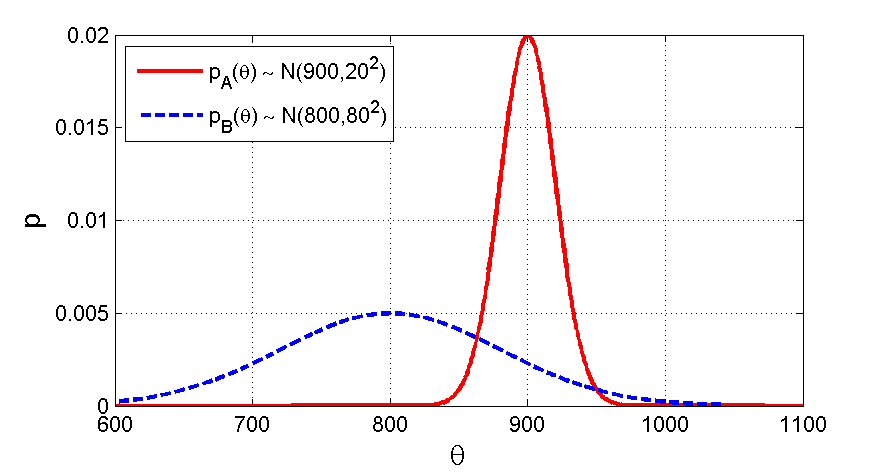
\includegraphics[width=130mm]{08_vorlesung/media/prior_A_Prior_B.png}
		\caption{\label{fig:Beispiel_1_a} Prior-Verteilungen für A und B}
	\end{center}
\end{figure}
Wir nehmen zunächst an, dass die physik. Konstante einmal beobachtet wird mit 
dem Mittelwert $\theta = 850$ und der Standardabweichung 40, d.h. 
als Likelihood der Messdaten haben wir eine Normalverteilung $l(\theta|X) \sim \mathcal{N}(850,40)$.
Abb.\ref{fig:Beispiel_1_b} zeigt die Wahrscheinlichkeitsdichtefunktion (engl.\ \textsl{probability density function}, kurz pdf) der Likelihood und Abb.\ref{fig:Beispiel_1_c} 
die Posteriorverteilung $p_\mathrm{A}(\theta|X)$ für den Beobachter A und die Posterior-Verteilung $p_\mathrm{B}(\theta|X)$ für den Beobachter B. Abb. \ref{fig:Beispiel_1_c} 
zeigt, dass Beobachter A nicht viel gelernt hat, während Beobachter B viel gelernt hat.

\begin{figure}[!h]
	\begin{center}
		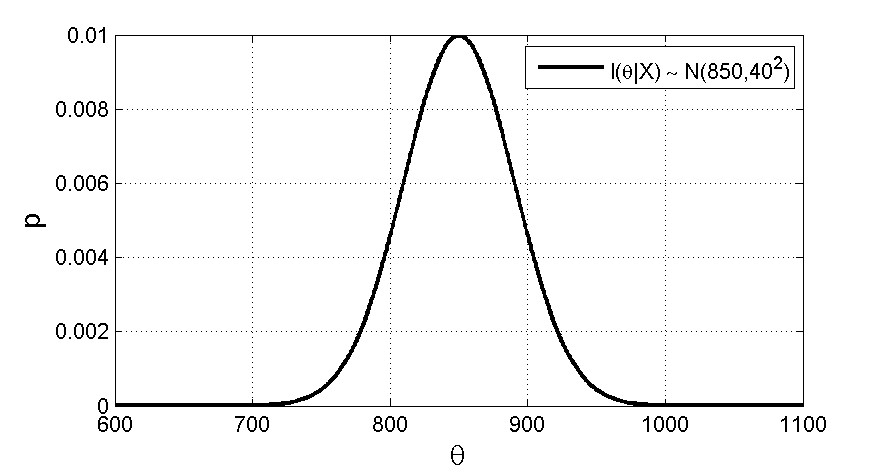
\includegraphics[width=130mm]{08_vorlesung/media/likelihood_1_Beobachtung.png}
		\caption{\label{fig:Beispiel_1_b} Standardisierte Likelihood
		für 1 Beobachtung mit x = 850}
	\end{center}
\end{figure}

\begin{figure}[!h]
	\begin{center}
		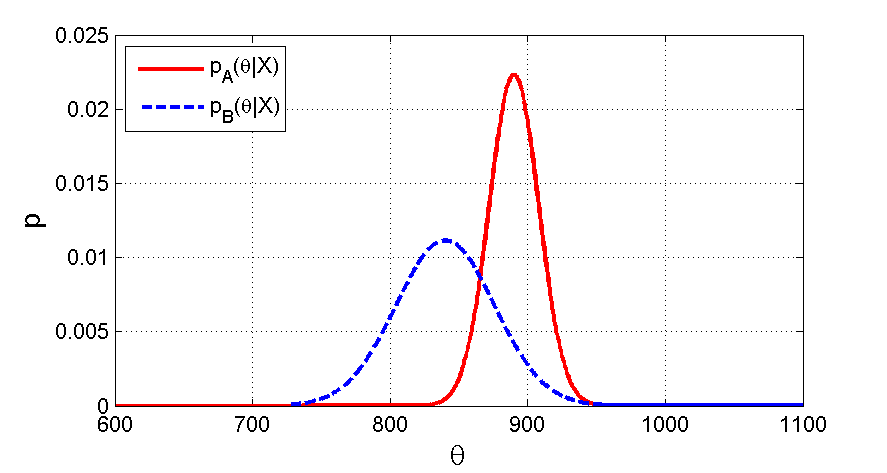
\includegraphics[width=130mm]{08_vorlesung/media/posterior_A_posterior_B.png}
		\caption{Posterior Verteilung für A und B 
		nach einer Beobachtung mit $\sigma_A = 17.9$ und $\sigma_B = 35.7$. D.h. A hat wenig gelernt, B hat viel gelernt.}
     	\label{fig:Beispiel_1_c}
	\end{center}
\end{figure}

Wenn sowohl der Prior $\theta \sim N(\theta_0,\sigma_0^2)$ als auch die 
Likelihood normalverteilt ist, dann ist auch der Posterior $p(\theta|X)$ normalverteilt mit $\mathcal{N}(\bar{\theta},\bar{\sigma}^2)$, wobei
\begin{equation}
\bar{\theta} = \frac{1}{w_0+w_1}(w_0 \theta_0 + w_1 x)\quad, \quad
\frac{1}{\bar{\sigma}^2}=w_0 + w_1 \\
\label{eq:prior_Normal}
\end{equation}
\[
\mathrm{mit} \quad \quad w_0 = \frac{1}{\sigma_0^2} \quad \mathrm{und} \quad w_1=\frac{1}{\sigma_1^2}
\]
Beweis dazu siehe weiter unten. \\
Mit $\bar{\sigma}^2$ bezeichnen wir hier die Varianz der Posterior 
und nicht die Varianz des Mittelwertes. D.h. durch die Beobachtung
wird meine Varianz upgedatet. Bei $J$ Beobachtungen wäre dann die Varianz $\bar{\sigma}^2$ des Posteriors die Kombination aus der
Varianz des Priors $\sigma_0^2$ und den Messungen $\sigma_j^2$:
\[
\frac{1}{\bar{\sigma}^2} = \left( \sum_{j=1}^{J} 
\frac{1}{\sigma_j^2}\right) + \frac{1}{\sigma_0^2} 
\] 
Der Posterior Mittelwert $\bar{\theta}$ ist das gewichtete Mittel des Prior-Mittelwertes
und des Mittelwertes $x$ der Beobachtung $X$. 

Für den Beobachter A ergibt sich der Mittelwert des Posteriors zu:
\[
\bar{\theta}_\mathrm{A} = \frac{1}{1/20^2+1/40^2}\left( \frac{1}{20^2}\cdot 900 + 
 \frac{1}{40^2}\cdot 850  \right) = 890
\]
Die Standardabweichung ergibt sich zu: 
\[
\frac{1}{\bar{\sigma}_\mathrm{A}^2}=\frac{1}{20^2} + \frac{1}{40^2} \Rightarrow
\bar{\sigma}_\mathrm{A} = 17.9
\]
Die Ergebnisse sind in Tab.\ref{tab:Ergebnisse des Beispiels} zusammengefasst.
\begin{table}[!h]
	\caption{Zusammenfassung der Ergebnisse für Beobachter A und B. A lernt 
	wenig. B lernt viel.}
	\centering
	\begin{tabular}{c c c}  \hline 
		Prior Verteilung & Likelihood von den Daten & Posterior Verteilung\\
		\hline
		A & A & A \\
		$\theta \sim N(900, 20^2)$ &$N(850,40^2)$ & $\theta \sim N(890, 17.9^2)$ \\ 
		B &B & B \\
		$\theta \sim N(800, 80^2)$ &$N(850,40^2)$ & $\theta \sim N(840, 35.7^2)$ \\
		\hline 
	\end{tabular}
	\label{tab:Ergebnisse des Beispiels}
\end{table}

Nehmen wir jetzt an, dass 99 weitere unabhängige Messungen zur Bestimmung der 
phys. Konstante gemacht werden mit einem Mittelwert $\bar{x} = 1/100 \cdot \sum_{j=1}^{100}$ für 100 Beobachtungen mit Mittelwert 870. Die Likelihood-Funktion von $\theta$ bei $J$ unabhängigen Beobachtungen, die normalverteilt $N(\theta, \sigma^2)$ sind, ist gegeben durch:
\[
l(\theta|X) \propto \left( \frac{1}{\sqrt{2\pi}\sigma}\right)^J 
\exp \left[-\; \frac{1}{2\sigma^2}\sum_{j=1}^{J}(X_j-\theta)^2\right] 
\]
Da 
\[
\sum_{j=1}^{J} (X_j-\theta)^2 = \sum_{j=1}^{J} (X_j-\bar{(X)})^2+J(\theta-\bar{(X)})^2
\]
und die gegebenen Daten $\sum(X_j-\bar{Y})^2$ eine feste Konstante ist, so ist
die Likelihood:
% Likelihood des Erwartungswertes
\begin{equation}
l(\theta|X) \propto 
\exp \left[-\; \frac{1}{2} \left(\frac{\theta-\bar{X}}{\sigma / \sqrt{(J)}}
\right)^2\right]
\label{eq:Likelihood_Stichprobenumfang_J} 
\end{equation}
D.h. dies ist eine Normalverteilung zentriert bei $\bar{X}$ mit Standardabweichung des Mittelwertes
$\sigma / \sqrt{J}$.
Im gegebenem Beispiel ist die Likelihood die Normalverteilung mit dem Mittelwert
$\bar{X} = 870$ und der Standardabweichung des Mittelwertes $\sigma/\sqrt{(J)} = 40 / \sqrt{100} = 4$.
Dies ist in Abb. \ref{fig:Beispiel_1_d} gezeigt.

\begin{figure}[!h]
	\begin{center}
		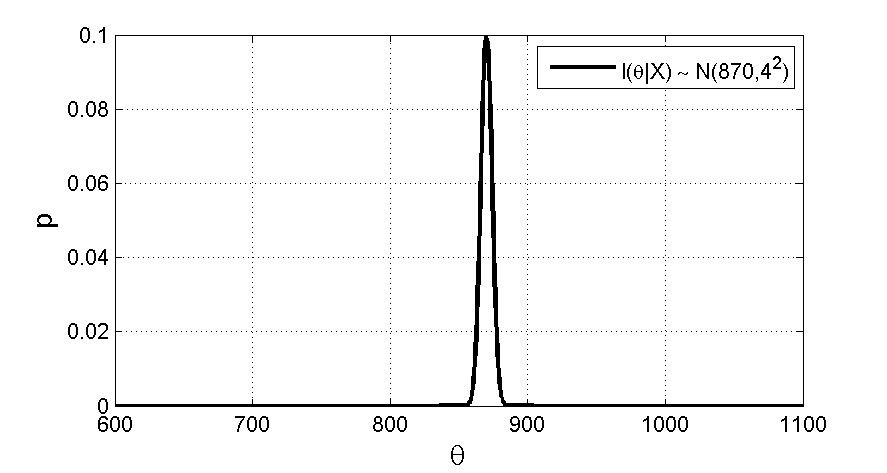
\includegraphics[width=130mm]{08_vorlesung/media/likelihood_100_Beobachtung.png}
		\caption{Standardisierte Likelihood
		für 100 Beobachtungen mit $\bar{X} = 870$}
	    \label{fig:Beispiel_1_d}
	\end{center}
\end{figure}

Mit der Formel in Gl.(\ref{eq:prior_Normal}) errechnen sich die Posterior-Verteilungen 
von A und B zu $N(871.2,3.9^2)$ und $N(869.8,3.9995^2)$.
Diese sind in Abb.\ref{fig:9_Beispiel_1_e} dargestellt. 

\begin{figure}[!h]
	\begin{center}
		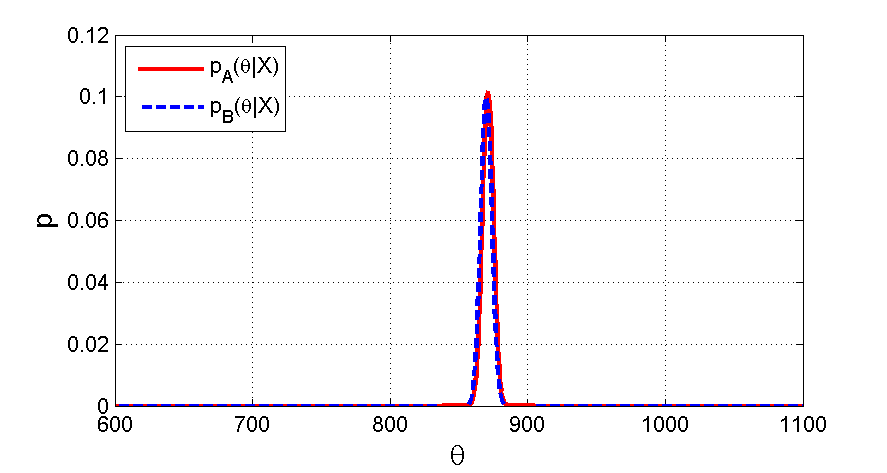
\includegraphics[width=130mm]{08_vorlesung/media/posterior_A_posterior_B_100_Beobachtungen}
		\caption{Posterior-Verteilungen für A und B nach 100 Beobachtungen}
		\label{fig:9_Beispiel_1_e} 
	\end{center}
\end{figure}

Nach 100 Beobachtungen sind die Beobachter A und B fast in Übereinstimmung.
Das Prior-Wissen von A und B spielt fast keine Rolle mehr. In Tabelle 
\ref{tab:Ergebnisse des Beispiels_bei_100_Stichproben} sind die Ergebnisse
dargestellt.

\begin{table}[!h]
	\caption{Zusammenfassung der Ergebnisse für Beobachter A und B bei 100
	Beobachtungen. Vorwissen von Beobachter A und B spielt fast keine Rolle mehr}
	\centering
	\begin{tabular}{c c c}  \hline 
		Prior Verteilung & Likelihood von den Daten & Posterior Verteilung\\
		\hline
		A & A & A \\
		$\theta \sim N(900, 20^2)$ &$N(870,4^2)$ & $\theta \sim N(871.2, 3.9^2)$ \\ 
		B &B & B \\
		$\theta \sim N(800, 80^2)$ &$N(870,4^2)$ & $\theta \sim N(869.8, 3.995^2)$ \\
		\hline 
	\end{tabular}
	\label{tab:Ergebnisse des Beispiels_bei_100_Stichproben}
\end{table}
\newpage
\textbf{Anhang: Herleitung von Gl.(\ref{eq:prior_Normal})}

Im Folgenden wollen wir noch die Gl.(\ref{eq:prior_Normal}) herleiten, mit der 
wir die Posterior berechnen können, wenn die Prior-Verteilung und die Likelihood 
normalverteilt sind.
Wir nehmen an, dass die Prior normalverteilt ist mit: 
\begin{equation}
p(\theta) = \frac{1}{\sqrt{2\pi}\sigma_0}\exp\left[-\quad 
\frac{1}{2}\left(\frac{\theta-\theta_0}{\sigma_0}\right)^2\right], 
\quad -\infty < \theta < \infty
\end{equation}
Die Likelihood-Funktion von $\theta$ ist ebenfalls normalverteilt: 
\begin{equation}
l(\theta|X) \propto \exp\left[-\quad 
\frac{1}{2}\left(\frac{\theta-X}{\sigma_1}\right)^2\right]
\end{equation}
Die Posterior-Verteilung erhalten wir dann: 
\begin{equation}
p(\theta|X) = \frac{p(\theta)\; l(\theta|X)}{\int_{-\infty}^{\infty} 
p(\theta)\;l(\theta|X))d\theta} = \frac{f(\theta|X)}{\int_{-\infty}^{\infty}
f(\theta|X) d\theta}
\end{equation}
mit 
\begin{equation}
f(\theta|X) = \exp \; \left\lbrace  -\; \frac{1}{2} 
\left[\left(\frac{\theta - \theta_0}{\sigma_0}\right)^2 + 
\left(\frac{\theta -X}{\sigma_1}\right)^2\right]  \right\rbrace 
\end{equation}
Unter der Verwendung der Identität
\begin{equation}
A(z-a)^2+B(z-b)^2 = (A+B)(z-c)^2 + \frac{AB}{A+B}(a-b)^2
\end{equation}
mit 
\begin{equation}
c = \frac{1}{A+B}(A\;a+B\;b)
\end{equation}
können wir den folgenden Ausdruck wie folgt schreiben: 
\begin{equation}
\left( \frac{\theta-\theta_0}{\sigma_0}\right)^2 + 
\left(\frac{\theta-X}{\sigma_1}\right)^2 = 
(\sigma_0^{-2} + \sigma_1^{-2}) \; (\theta - \bar{\theta})^2 + d
\end{equation}
wobei
\[
\bar{\theta} = \frac{1}{\sigma_0^{-2}+\sigma_1^{-2}}
(\sigma_0^{-2}\theta_0 + \sigma_1^{-2} X)
\]
und $d$ ist konstant, d.h. unabhängig von $\theta$. 
Somit 
\begin{equation}
f(\theta |X) = \exp \left( -\; \frac{d}{2}\right) \exp [-\; 1/2 \cdot 
(\sigma_0^{-2}+\sigma_1^{-2})(\theta - \bar{\theta})^2]
\end{equation}

so dass
\begin{equation}
\begin{array}{rcl}
\int_{-\infty}^{\infty} f(\theta|X) d \theta & = & 
\exp \left( -\; \frac{d}{2} \right) \cdot \int_{-\infty}^{\infty} 
\exp \left[ - \; \frac{1}{2} (\sigma_0^{-2}+ \sigma_1^{-2})(\theta - \bar{\theta})^2
\right] d \theta \\
&=& \sqrt{2 \pi} (\sigma_0^{-2}+\sigma_1^{-2})^{-1/2} \exp (-d/2) 
\end{array}
\end{equation}
Es folgt daraus, dass 
\begin{equation}
p(\theta|X) = \frac{(\sigma_0^{-2}+\sigma_1^{-2})^{1/2}}{\sqrt{2\pi}}
\exp \left[- 1/2 \cdot (\sigma_0^{-2}+\sigma_1^{-2})(\theta-\bar{\theta})^2)\right]
\end{equation}
mit der Normalverteilung
\begin{equation}
N\left[\bar{\theta}, \; (\sigma_0^{-2} + \sigma_1^{-2})^{-1} \right]
\end{equation}

\textbf{Anhang: Octave/Matlab-Skript zum Beispiel \glqq Physikalische Konstante\grqq}

\begin{verbatim}
% by Ehret, 2019-12-10
clear all; close all;
% Bayes for a physical constant

% Definition der X-Werte
X = linspace(600,1100,1000);

% Beispiel 
% Prior-Verteilung des Beobachters A
% Normalverteilt mit mu_A = 900 und sigma_a = 20
mu_A = 900;
sigma_A = 20;
DeltaX = X(2)-X(1);
p_A = normpdf(X,mu_A, sigma_A);

% Prior-Verteilung des Beobachters B
% Normalverteilt mit mu_B = 800 und sigma_a = 80
mu_B = 800;
sigma_B = 80;
p_B = normpdf(X,mu_B, sigma_B);

% Plotten der Prior-Verteilungen von A und B
figure(1)
plot(X,p_A,'r-','linewidth',2)
hold on;
plot(X,p_B,'b--','linewidth',2)
grid on;
legend('p_A(theta) ~ N(900,20^2)','p_B(theta) ~ N(800,80^2)', ...
'Location','NorthWest')
xlabel('\theta','fontsize',14)
ylabel('p','fontsize',14)

% Annahme der Likelihood (Messung) als Normalverteilung mit l ~ N(850,40^2 ) 
mu_likeli = 850;
sigma_likeli = 40;
likelihood = normpdf(X,mu_likeli, sigma_likeli);

% Plotten der Likelihood
figure(2)
plot(X,likelihood,'k-','linewidth',2)
grid on;
legend('l(theta|X) ~ N(850,40^2)')
xlabel('\theta','fontsize',14)
ylabel('p','fontsize',14)

% Berechnung der Posterior für eine Beobachtung für A und B
% Posterior ~ Prior  x Likelihood
p_post_A_1 = p_A .* likelihood;
p_post_B_1 = p_B .* likelihood;

% Normierung des posterior mit Normierungskonstante 
% Nicht ganz korrekt, da eigentlich 
% von -\inf bis +\inf integriert bzw. summiert werden müsste

const_post_A1 = 1/sum(p_post_A_1*DeltaX);
p_post_A_1 = const_post_A1 * p_post_A_1 ;

const_post_B1 = 1/sum(p_post_B_1*DeltaX);
p_post_B_1 = const_post_B1 * p_post_B_1 ;

% Plotten der Posterior
figure(3)
plot(X,p_post_A_1,'r-','linewidth',2)
hold on;
plot(X,p_post_B_1,'b--','linewidth',2)
grid on;
legend('p_A(theta|X)','p_B(theta|X)', ...
'Location','NorthWest')
xlabel('\theta','fontsize',14)
ylabel('p','fontsize',14)

% Jezt besteht die Likelihood aus 100 Stichproben
% Berechnung der Posterior für 
% Bei hundert Stichproben kann die Verteilung schmaler werden
% also z.B. Dann mit sigma_likeli_100 = sigma_likeli / root (N)
N = 100;
sigma_likeli_100 = sigma_likeli / sqrt(N);
% Als Mittelwert wir angenommen:
mu_likeli_100 = 870;

% Likelihood Funktion für 100 Stichproben
likelihood_100 = normpdf(X,mu_likeli_100, sigma_likeli_100);

figure(4)
plot(X,likelihood_100,'k-','linewidth',2)
grid on;
legend('l(theta|X) ~ N(870,4^2)')
xlabel('\theta','fontsize',14)
ylabel('p','fontsize',14)

% Berechnung der Posterior für 100 Beobachtung für A und B
p_post_A_100 = p_A .* likelihood_100;
p_post_B_100 = p_B .* likelihood_100;

% Normierungskonstante % Nicht ganz korrekt, da eigentlich 
% von -\inf bis +\inf integriert bzw. summiert werden müsste
const_post_A_100 = 1/sum(p_post_A_100*DeltaX);
p_post_A_100 = const_post_A_100 * p_post_A_100 ;

const_post_B_100 = 1/sum(p_post_B_100*DeltaX);
p_post_B_100 = const_post_B_100 * p_post_B_100 ;

figure(5)
plot(X,p_post_A_100,'r-','linewidth',2)
hold on;
plot(X,p_post_B_100,'b--','linewidth',2)
grid on;
legend('p_A(theta|X)','p_B(theta|X)', ...
'Location','NorthWest')
xlabel('\theta','fontsize',14)
ylabel('p','fontsize',14)
\end{verbatim} 
\newpage
\subsection{Priorverteilungen}
Das Bayes-Theorem verwendet eine Prior-Verteilung, also ein Vorwissen über die zu schätzenden Modellparameter.
Für Situationen, in denen es im wesentlichen kein Vorwissen gibt, wird eine einfache Rechteckverteilung als Prior angesetzt, was bedeutet, dass die Wahrscheinlichkeit innerhalb eines vorgegebenen Intervalls $[\theta_\mathrm{li},\theta_\mathrm{re}]$ konstant ist:
\[
p(\theta) = \left\{\begin{array}{lll}
\textrm{const.} & \textrm{falls} & \theta \in [\theta_\mathrm{li},\theta_\mathrm{re}]\\
0 & \textrm{sonst.} &
\end{array}\right.
\]
Dieser Ansatz ist mit Vorsicht zu verwenden:
Die Posterior kann mehrere lokale Maxima, die ähnlich groß sind, aufweisen.
Sie kann auch ihrerseits nahezu rechteckverteilt sein.
Je nach Modell kann dieser Ansatz mit ungeschickt gewähltem Intervall
$[\theta_\mathrm{li},\theta_\mathrm{re}]$ zu numerischen Problemen führen.
Besonders problematisch ist die Situation, wenn mangels Vorwissen für die Intervallgrenzen
oder für eine der beiden Intervallgrenzen der Grenzübergang ins Unendliche vorgenommen wird.
Das kann dann dazu führen, dass kein physikalisch oder statistisch sinnvoller
Erwartungswert bestimmt werden kann. 

Ein Beispiel hierfür ist die Bestimmung der Fläche eine Rechteckes $F=a \cdot b$.
Wenn wir kein Wissen über das Verhältnis der Seitenlängen $a$ und $b$ 
haben, dann würden wir zunächst sagen, dass alle Verhältnisse $R = a/(a+b)$ gleichverteilt sind. Wir können dies auch als $R=1/(1+b/a))$
umschreiben. Für $b/a \rightarrow 0$ ergibt sich für das Verhältnis 
$R=1$, für $b/a \rightarrow \infty$ ergibt sich für das Verhältnis
$R=0$. Wir können somit anehmen, dass die Verhältnisse zwischen 
$0$ und $1$ gleichmäßig verteilt sind, wenn wir keine Vorkenntnisse 
haben. 
Umgekehrt,wenn wir nichts über die Fläche wissen, würden wir annehmen, dass alle Flächen gleichverteilt sind. Beide Priors sind in Abb. \ref{fig:Beispiel_Flaechenbestimmung_Verteilungen01} dargestellt.

\begin{figure}[!h]
 	\begin{center}
		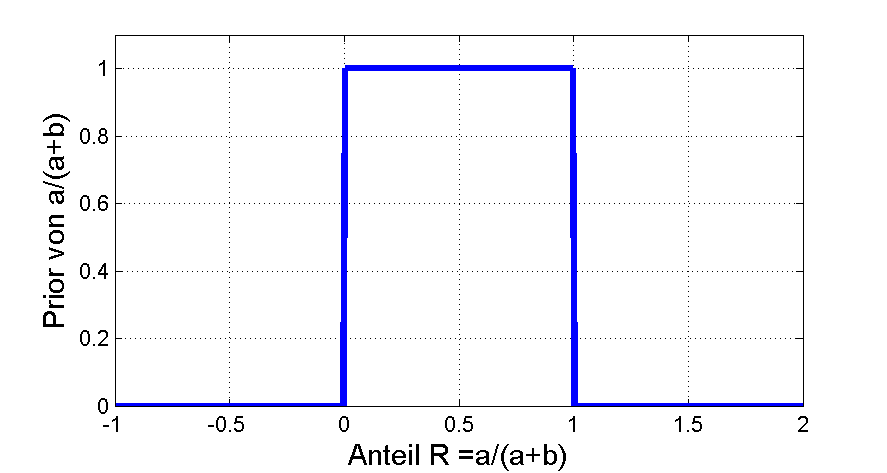
\includegraphics[width=80mm]{08_vorlesung/media/prior_des_Anteils_1.png}
		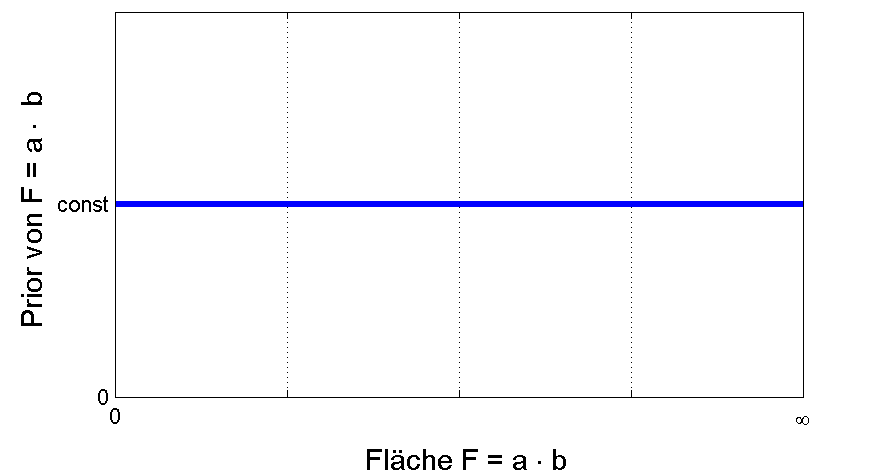
\includegraphics[width=80mm]{08_vorlesung/media/prior_der_Flaeche_1.png}
		\caption{Plausible Priors für den Anteil $a/(a+b)$ und die Fläche $F = a\cdot b.$ Beide Priors sind jedoch nicht konsistent zueinander.} 
		\label{fig:Beispiel_Flaechenbestimmung_Verteilungen01} 
	\end{center}
\end{figure}
\begin{figure}[!ht]
	\begin{center}
		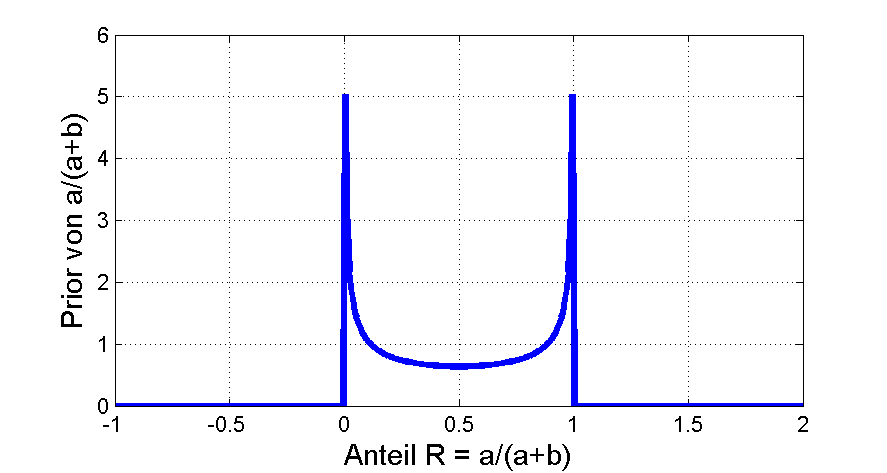
\includegraphics[width=80mm]{08_vorlesung/media/prior_des_Anteils_2.png}
		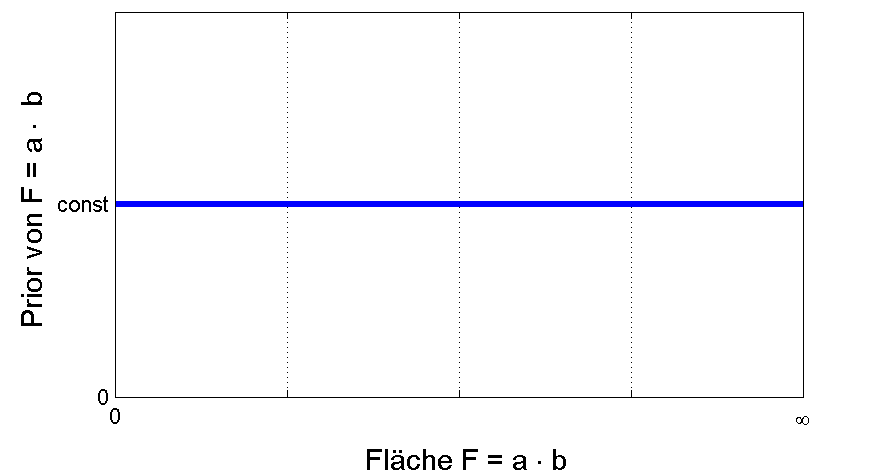
\includegraphics[width=80mm]{08_vorlesung/media/prior_der_Flaeche_2.png}
		\caption{ links: Jeffreys Prior für den Anteil $R=a/(a+b)$, eine Betaverteilung (0,5;0,5), rechts: Jeffreys Prior für den Erwartungswert einer normalverteilten Größe, hier ist dies die Fläche $F = a\cdot b.$ Beide Priors sind jetzt konsistent zueinander.}
		\label{fig:Beispiel_Flaechenbestimmung_Verteilungen02}
	\end{center}
\end{figure}
Wenn nun der Anteil $R=0$ ist, so muss auch die Fläche $F=0$ sein. 
Wenn der Anteil $R=1$ ist, so muss die Fläche $F=\infty$ sein. 
Bei $a=b$ ergibt sich ein Anteil $R=0.5$. Wenn wir die Priorverteilung
des Anteiles anschauen, so liegt der Anteil zu 50\% zwischen $0$
und $0.5$. Dies würde auch bedeuten, dass 50\% der Fläche zwischen
$F=0$ und $F=a^2= b^2$ liegen müssten. Dies steht jedoch im Widerspruch
zu der uniformen Annahme in Abb.~\ref{fig:Beispiel_Flaechenbestimmung_Verteilungen01}. 
Hier sind nicht 50\% der Fläche zwischen $[0,a^2=b^2]$ und 50\%
zwischen $[a^2=b^2,\infty]$.
Somit haben wir hier einen Widerspruch.
Deshalb hat sich hier Jeffrey \cite{Hel08} etwas einfallen lassen, 
er schlägt für den Prior des Anteiles, eine Beta-Verteilung
mit $\alpha = \beta = 0.5 $ vor, wie sie Abb. \ref{fig:Beispiel_Flaechenbestimmung_Verteilungen02} dargestellt ist. Nun haben wir in Abb.\ref{fig:Beispiel_Flaechenbestimmung_Verteilungen02} 
zwei in sich konsistente Prior-Verteilungen.
Unwissenheit kann also nicht grundsätzlich durch eine uniforme Verteilung
dargestellt werden \cite{Tsc14}.

Die Betaverteilung ist eine stetige Wahrscheinlichkeitsverteilung über dem Intervall $( 0 , 1 )$.
Die Beta-Verteilungsdichte ist definiert durch (siehe z.~B. Wikipedia): 
\[
p(X) = \frac{1}{B(\alpha,\beta)} X^{\alpha-1}(1-X)^{\beta-1}.
\]
Außerhalb des Intervalls $(0,1)$ wird sie durch $p(X)=0$ fortgesetzt. 
Für $\alpha,\beta \geq 1$ lässt sich $(0,1)$ durch $[0,1]$ ersetzen. Die Betaverteilung besitzt die reellen Parameter $\alpha$ und $\beta$. Um ihre Normierbarkeit zu garantieren, wird $\alpha,\beta > 0$ gefordert.

Der Vorfaktor $1/B(\alpha,\beta)$ dient der korrekten Normierung. Der Ausdruck
\[B(\alpha,\beta) = \frac{\Gamma(\alpha) \Gamma(\beta)}{\Gamma(\alpha+\beta)} = \int_0^1 u^{\alpha-1} (1-u)^{\beta-1}\, \mathrm{d}u 
\]
steht für die Betafunktion, nach der die Verteilung benannt ist. Dabei bezeichnet $\Gamma$ die Gammafunktion.

Einige nützliche Priors sind beispielhaft in Tab.\ref{tab:Einige_Priors} dargestellt.

\begin{table}[!htbp]
	\caption{Häufig verwendete Priors.}
	 \vspace*{1ex}
	\centering
	\begin{tabular}{m{3cm} |m{3cm} m{4.5cm}| m{3cm}}  \hline 
		Vorhandenes Vorwissen & PDF \hspace{1em} und & Illustration & $x$ und $u(x)$\\ 
		\hline \vspace*{2ex}
		Schätzwert $x$ und Standardunsicherheit $u(x)$ \vspace*{4ex} &
		Normal: $\mathcal{N} (x, u(x)^2)$ & 
				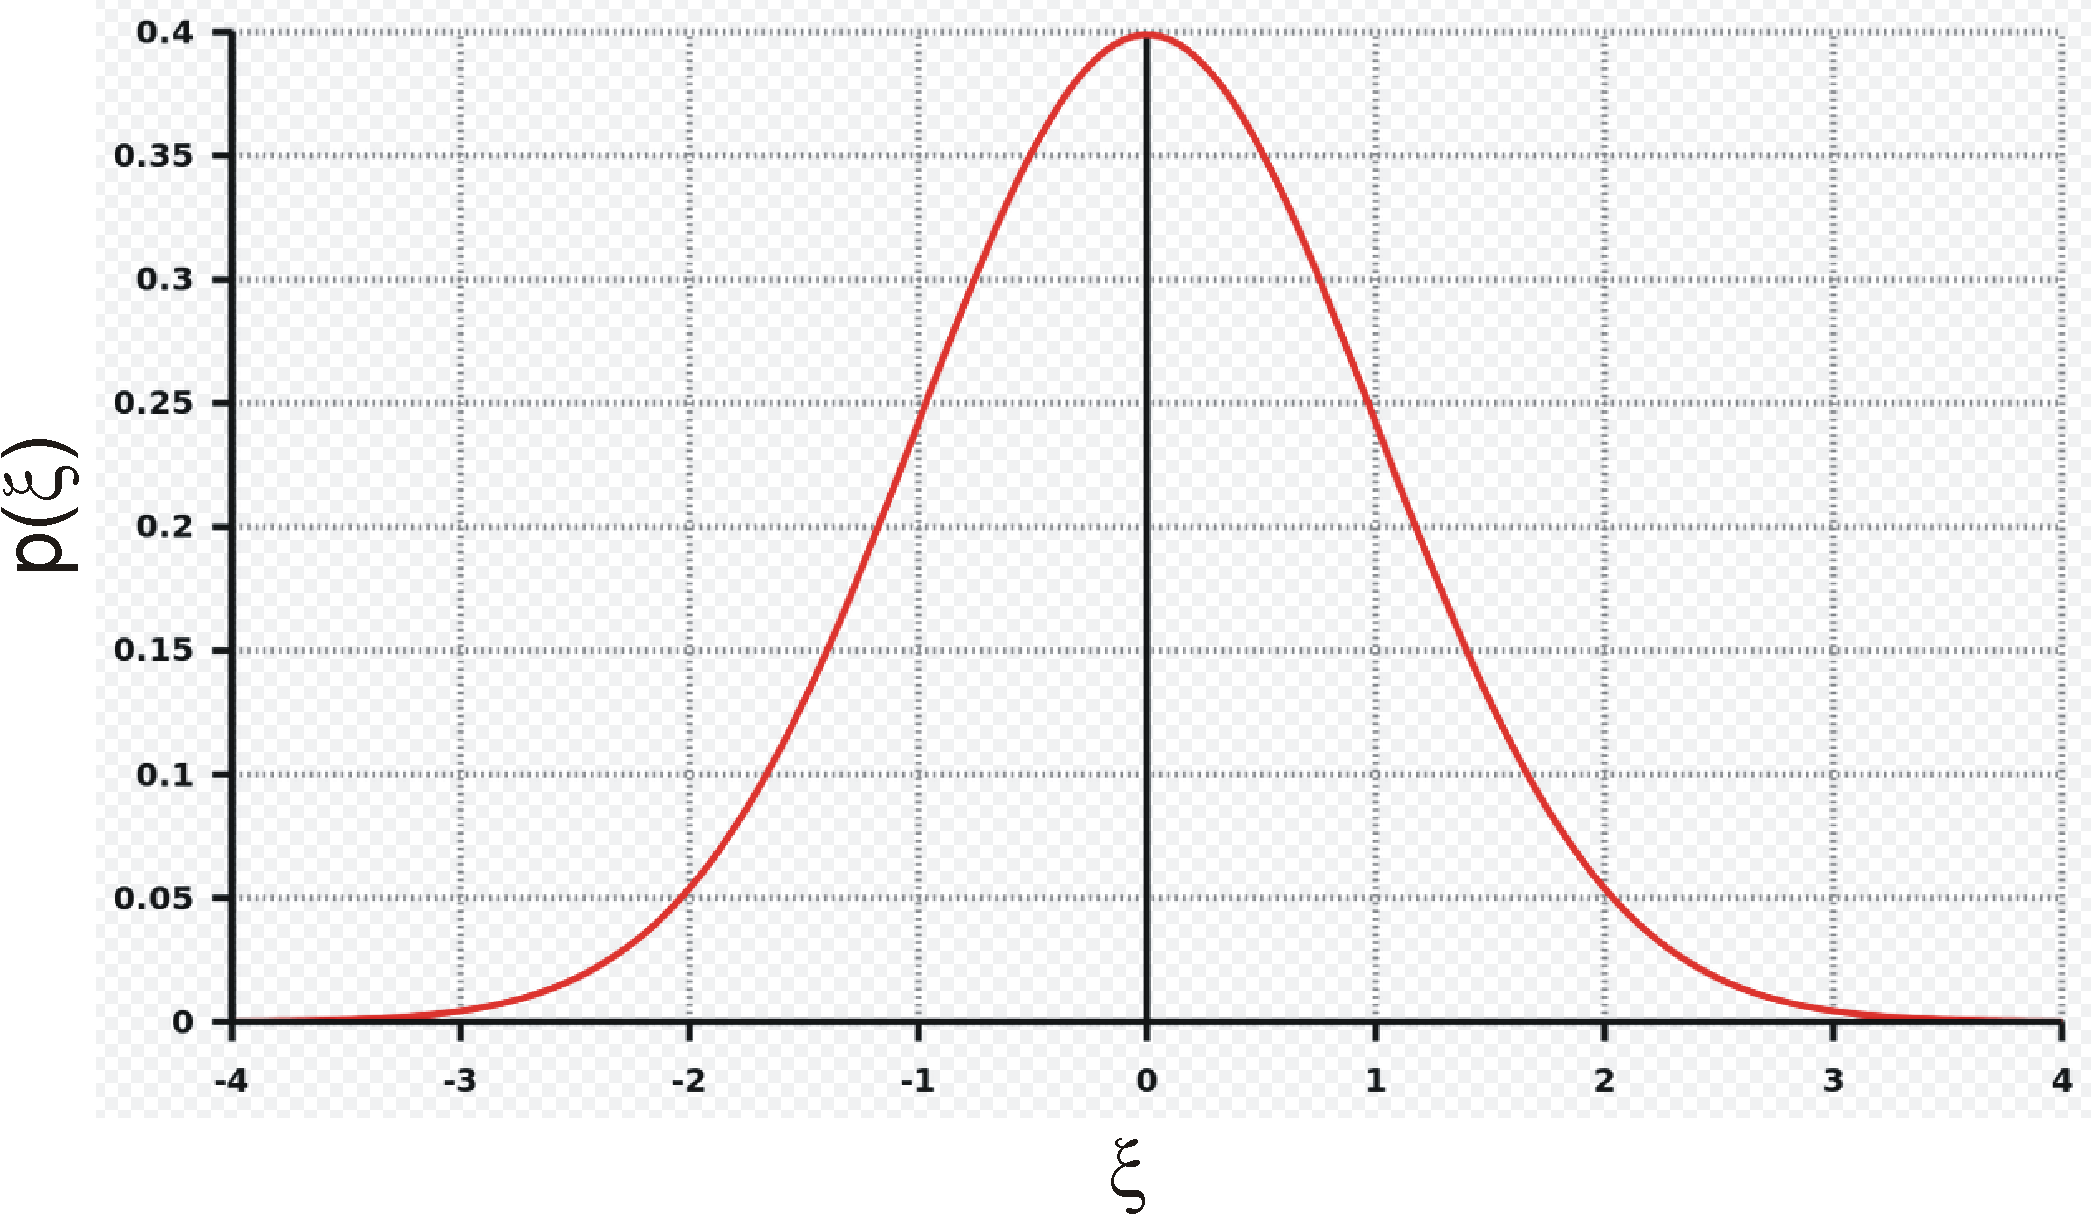
\includegraphics[width=40mm]{08_vorlesung/media/Prior_Normalverteilung.png}
	 & $x,\newline u(x)$ \\
	 \hline \vspace*{2ex}
	 Es sind schon vorhandene (historische) Werte bekannt. Der Erwartungswert und die Varianz ist jedoch unbekannt. \vspace*{4ex} &
	 Skalierte und \newline verschobene t-Verteilung $t_{n-1}(\bar \xi, s^2/n)$ & 
	 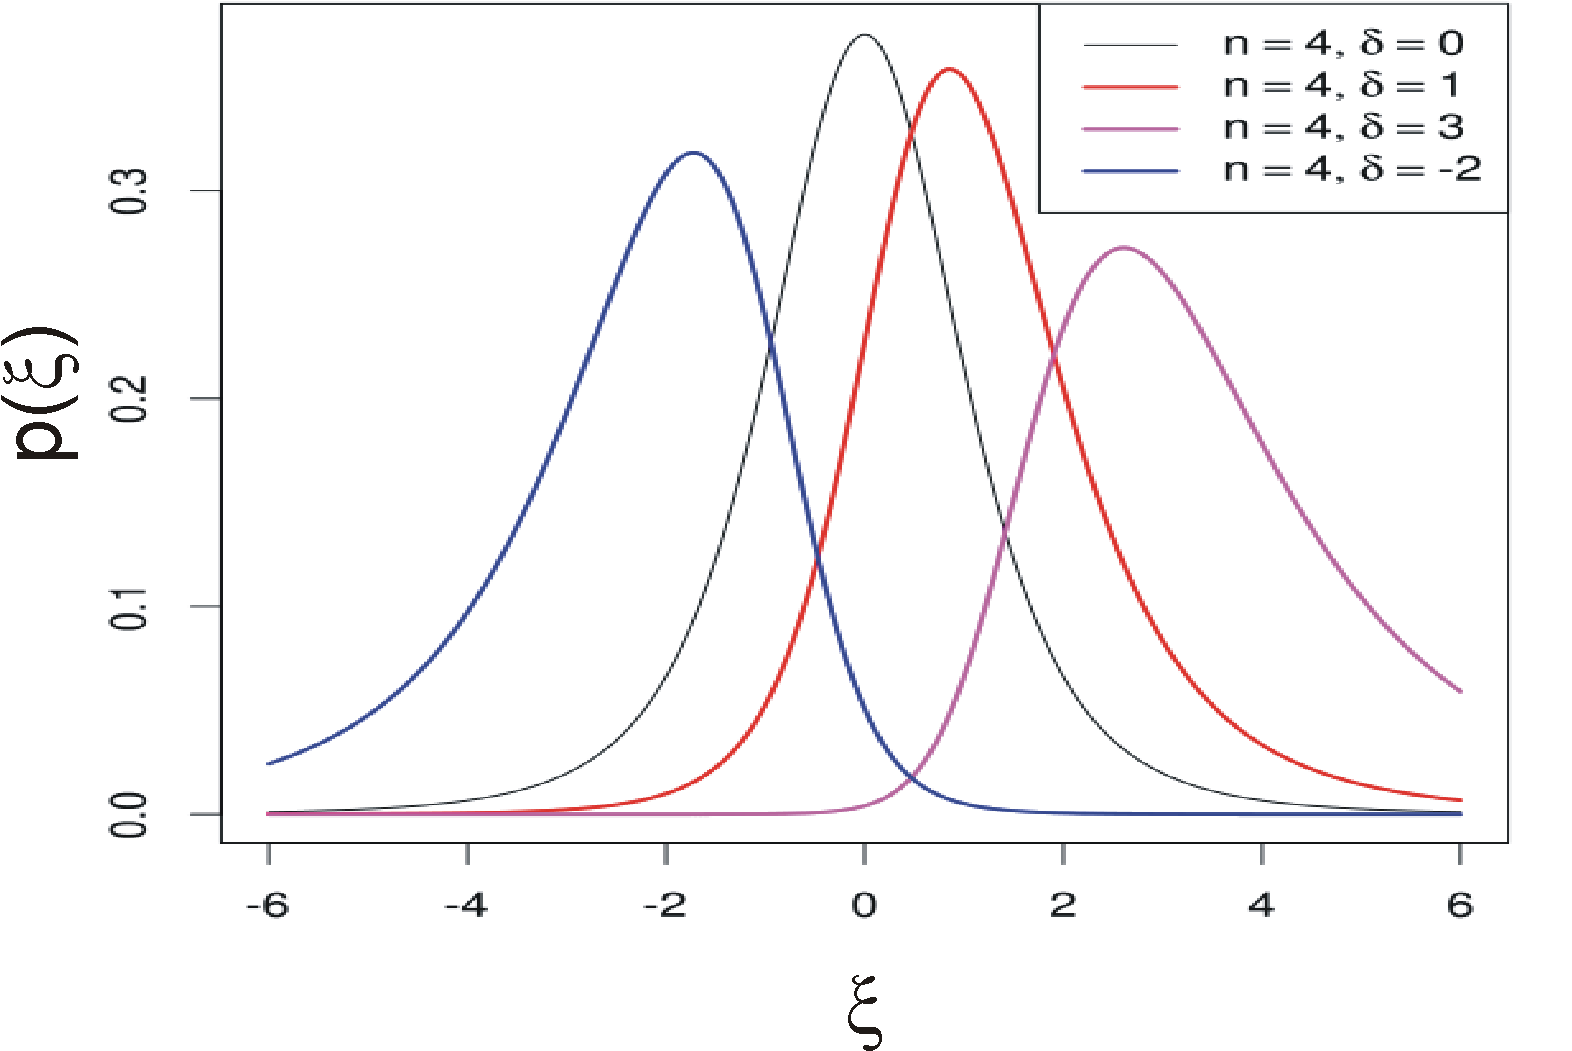
\includegraphics[width=40mm]{08_vorlesung/media/Prior_Studentverteilung.png}
	 & $x = \bar \xi, \newline u(x) = \left(\frac{n-1}{n-3}\right) \frac{s}{\sqrt{n}}$ \\
	 \hline \vspace*{6ex}
	 Kenntnisse über die Varianzen sind bekannt \vspace*{4ex} &
	
	 $\mathcal{X}^2 $ & 
	 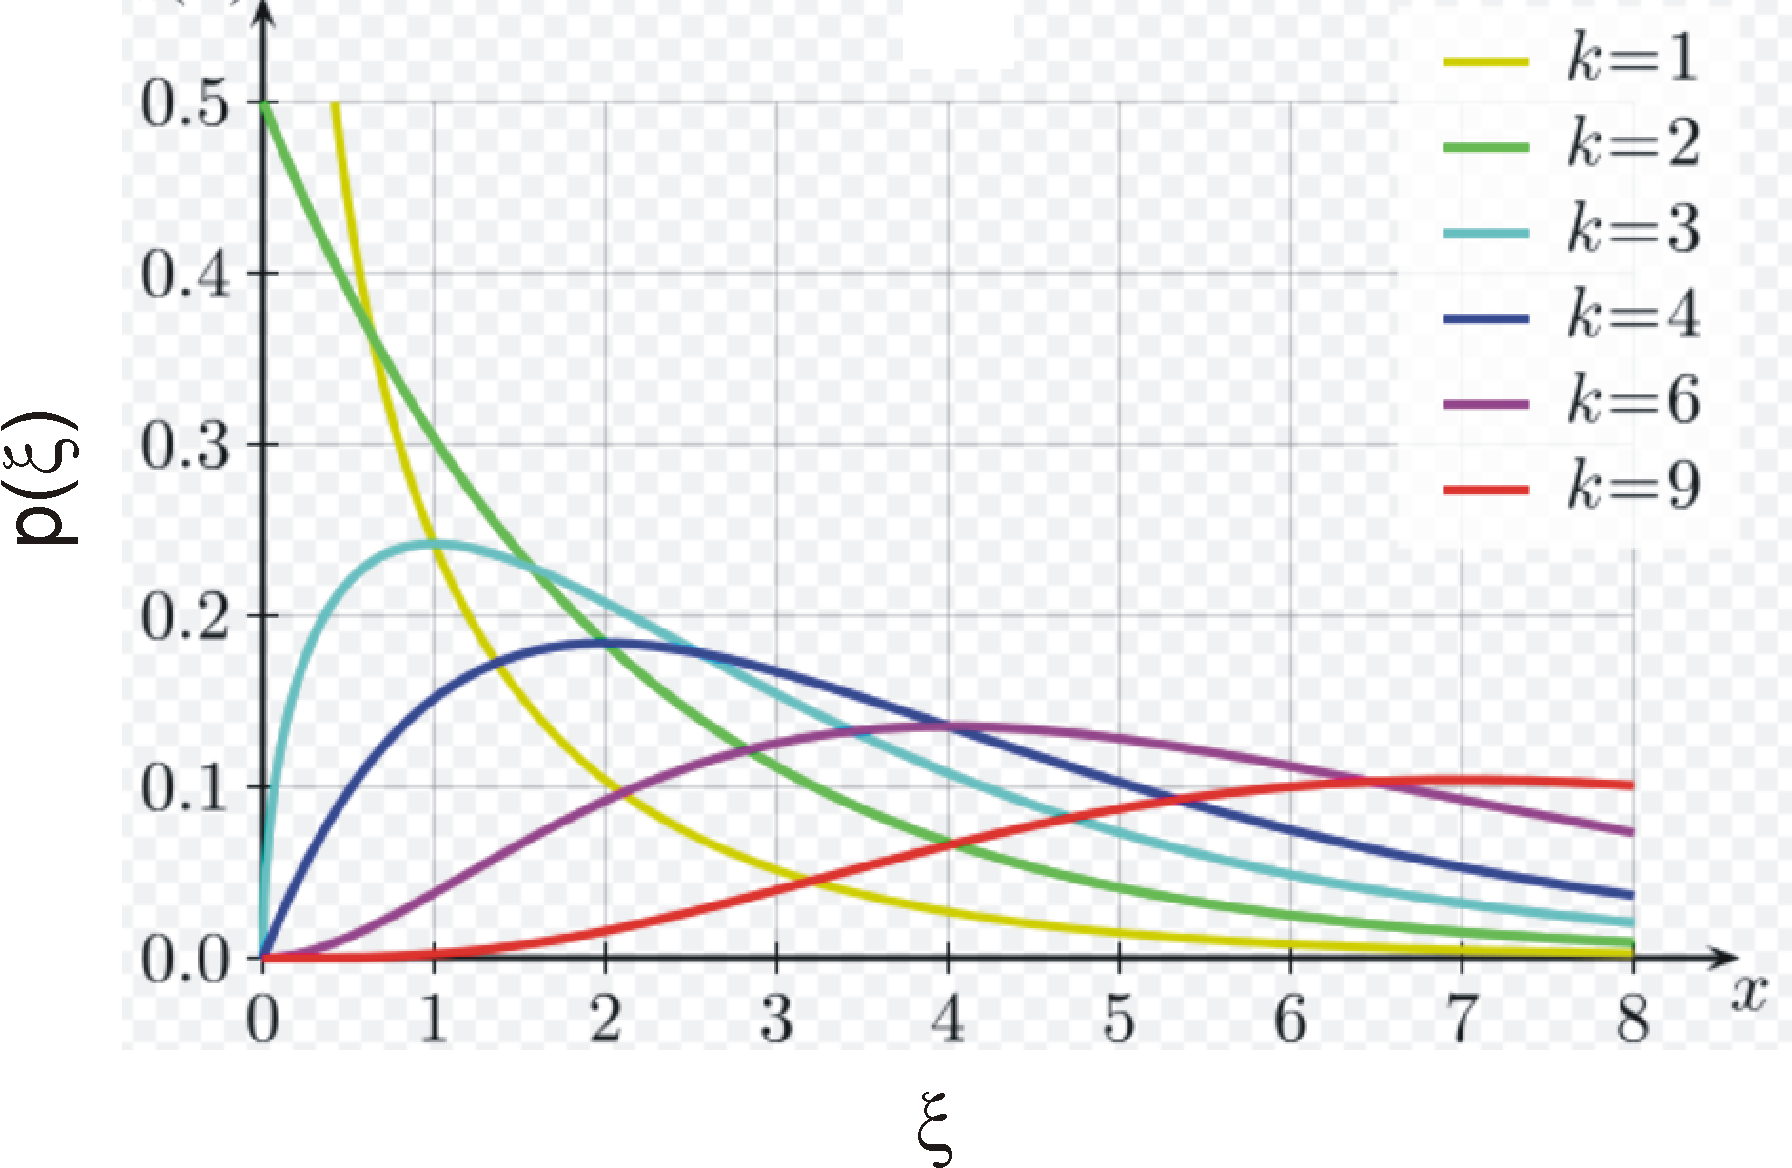
\includegraphics[width=40mm]{08_vorlesung/media/Prior_Chi2verteilung.png}
	 & $x, \newline u(x) $ \\
	  \hline \vspace*{4ex}
	Obere und untere Grenzen $a$, $b$ sind bekannt \vspace*{4ex} &
	Rechteck: $\mathcal{R}(a,b)$ & 
	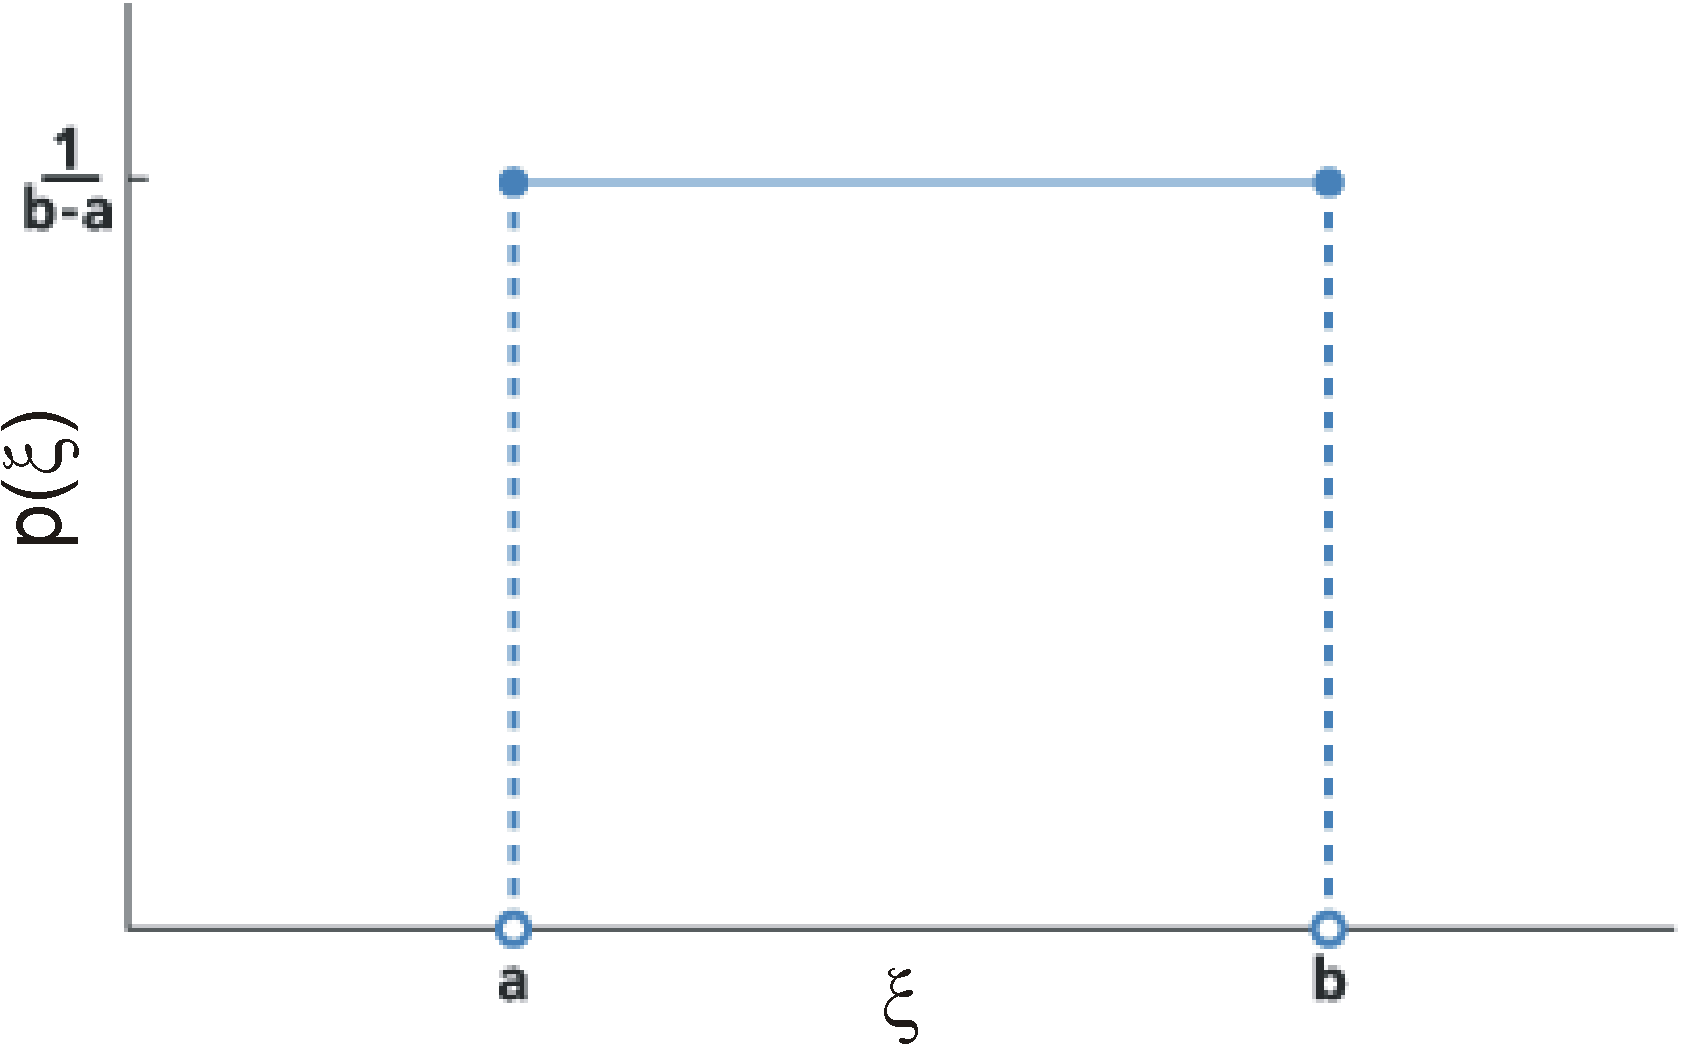
\includegraphics[width=40mm]{08_vorlesung/media/Prior_Rechteckverteilung.png}
	& $x = \frac{a+b}{2}, \newline u(x)=\frac{b-a}{\sqrt{12}} $ \\			 
				 
		\hline 
	\end{tabular}
	\label{tab:Einige_Priors}
\end{table}

\begin{comment}
\begin{figure}[!ht]
	\begin{center}
		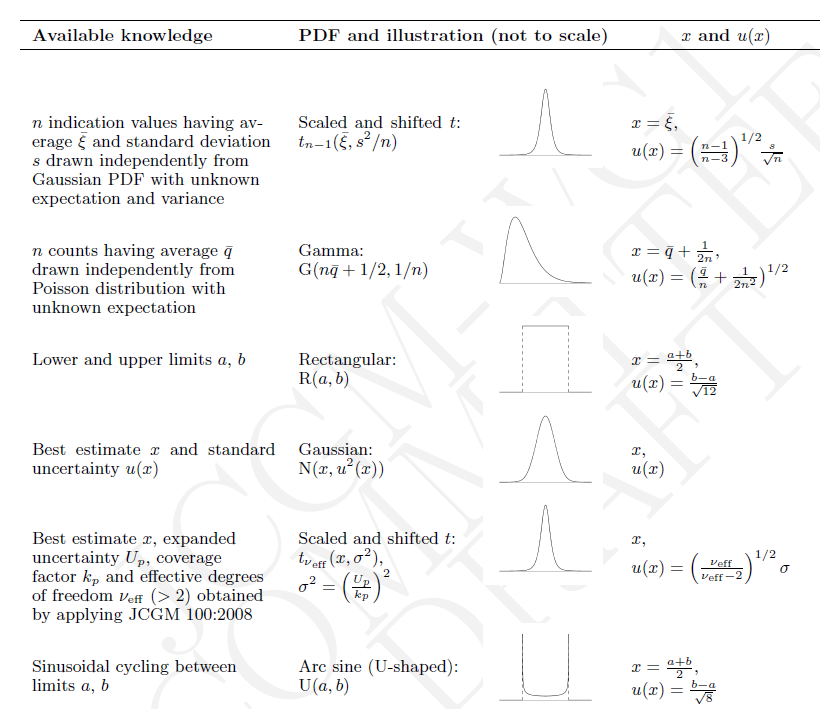
\includegraphics[width=150mm]{Bilder/PriorVerteilungen.png}
	%	\caption{ Priorverteilungen}
 	\label{fig:Priorverteilungen}
	\end{center}
\end{figure}
\end{comment}


\newpage
\textbf{Hinweise zur skalierten und verschobenen t-Verteilung als Prior} \\
(Wir bezeichnen hier die Anzahl der Beobachtungen mit $n$ und nicht mit $J$ um mit den Guides
zur Bestimmung der Messunsicherheit konsistent zu sein, also statt $\xi_{i,1}, \dots, \xi_{i,J}$ verwenden wir hier $\xi_{i,1}, \dots, \xi_{i,n}$)
Wenn angenommmen wird, dass wir aus $n$ Beobachtungen  $\xi_{i,1},\ldots,\xi_{i,n}$, die aus einer Gauß- bzw.
Normalverteilung (Erwartungswert und Varianz unbekannt) gezogen wurden und diese den Mittelwert $\bar{\xi}$
und die empirische Standardabweichung $s$ besitzt,  
so können wir eine mit der Varianz des Mittelwertes $s_i^2/n$ skalierte und 
um den Mittelwert $\bar \xi$ verschobene t-Verteilung mit $n-1$ Freiheitsgraden
annehmen: $t_{n-1}(\bar \xi, s_i^2/n)$.

Der beste Schätzwert für $X$ und die dazugehörige Varianz, die die beste Schätzung für die Unsicherheit darstellt, sind
\[
x = \bar{\xi} 
\]
\[
u(x_i) = \left(\frac{n-1}{n-3}\right)^{1/2} \; \frac{s_i}{\sqrt{n}}
\]
mit 
\[
s_i = \left[\frac{1}{n-1}\sum_{r=1}^{n}(\xi_{i,r}-\bar{\xi_i})^2\right]^{1/2}
\]
Eine Herleitung des Vorfaktors $\sqrt{\frac{n-1}{n-3}}$ ist z.~B. in \cite{Kac03} zu finden.  
\subsection{Posteriorverteilungen von Modellparametern}
Wir geben hier ein paar Beispiele für Posterior-Verteilungen an:

\textbf{(a) Priorverteilung
	ist konstant und die Varianz $\sigma$ der Messdaten $X$ ist bekannt}
\[
\mathrm{Priorverteilung:} \quad \quad p(\theta) \sim U(-\infty, + \infty)
\]
\[
\mathrm{Likelihood \;\; (siehe \; auch \; Gl.(  \ref{eq:Likelihood_Stichprobenumfang_J}})): \quad \quad l(\theta | X ) \sim N(\bar{X},
\sigma^2 /J)
\propto 
\exp \left[-\; \frac{1}{2} \left(\frac{\theta-\bar{X}}{\sigma / \sqrt{J}}
\right)^2\right]
\]
\[
\mathrm{Posteriorverteilung:}  \quad \quad p(\theta | X) 
\sim N(\bar{X},\sigma^2 / J)
\]
\textbf{(b) Priorverteilung
	ist normalverteilt und die Varianz $\sigma$ der Messdaten $X$ ist bekannt}
\[
\mathrm{Priorverteilung:} \quad \quad p(\theta) \sim 
N(\theta_0, \sigma_0^2)
\]
\[
\mathrm{Likelihood \;\; (siehe \;\;  auch \; Gl.  \ref{eq:Likelihood_Stichprobenumfang_J}}): \quad \quad l(\theta | X ) \sim N(\bar{X},
\sigma^2 /J)
\propto 
\exp \left[-\; \frac{1}{2} \left(\frac{\theta-\bar{X}}{\sigma / \sqrt{J}}
\right)^2\right]
\]
\[
\mathrm{Posteriorverteilung:}  \quad \quad p(\theta | X) 
\sim N(\bar{\theta},\bar{\sigma}^2)
\]
mit dem Erwartungswert 
\[
\bar{\theta} = \frac{\sigma_0^2\cdot \bar{X} + 
\frac{\sigma^2}{J}\cdot \theta_0}
{\sigma_0^2 + \frac{\sigma^2}{J}}
\]
und der Standardabweichung
\[
\bar{\sigma}^2 = \frac{\sigma_0^2 \cdot \frac{\sigma^2}{J}}
{\sigma_0^2 + \frac{\sigma^2}{J}}
\]

\textbf{(a) Priorverteilung
	ist normalverteilt und die Varianz $\sigma^2$ der Messdaten $X$ ist unbekannt} \\
Ist die Varianz der Messgröße unbekannt, so muss die Varianz noch geschätzt werden, z.~B. über die $\mathcal{X}^2$ -Verteilung.

\section{MU-Bestimmung mittels Posterior aus Bayesansatz}
\subsection{Bayessche Intervallschätzung}
Wie eine klassische Punktschätzung z.~B. mit MLE oder LS, so sagt auch eine bayessche nicht aus, wie nahe der Schätzwert dem wahren Wert kommt. Doch auch hier kann man ein Intervall angeben, die 
den wahren Wert mit einer gewissen Wahrscheinlichkeit enthalten. Der üblichen Sprachregelung folgend bezeichnen wir die Intervalle der Bayes-Statistik nicht als \textit{Vertrauens-} bzw. \textit{Konfidenz-Intervalle} sondern als 
\textit{Kredibilitätsintervalle}. (credibility: Glaubwürdigkeit, confidence: Vertrauen). 
Nicht weil das Wort credibility treffender wäre als das Wort confidence. Beide enstammen der Umgangssprache. Wir wählen den anderen Ausdruck, damit jederzeit klar wird, ob wir ein klassiches oder ein bayessches Intervall meinen. 
Der ISO-Guide verwendet den Begriff 
\textit{Überdeckungsintervall, engl. coverage interval},
das das Intervall angibt, das die Menge der wahren Werte einer Messgröße
mit einer angegeben Wahrscheinlichkeit enthält, auf der Grundlage der
verfügbaren Information \cite{VIM08}. 
(siehe zu den Begrifflichkeiten: Vertrauens-, Credible- und Überdeckungintervall auch die Ausführungen im Kapitel \glqq Messunsicherheitsfortpflanzung bei linearen
Modellen\grqq)
Den Wahrscheinlichkeitswert, den ein credible interval einschließt, bezeichnen wir als Kredibilitätsniveau $\gamma.$

Beispiel: Symmetrische/ nichtsymmetrische Verteilungen

Bei symmetrischen Posterior-Verteilungen wird in der Regel 
das symmetrische Intervall genommen. So ist in Abb. \ref{fig:Beispiel_Bestimmung_CredibleIntervall}  das 95\%ige Intervall 
einer Normalverteilung $N(10,4^2)$ dargestellt. 
Die untere und obere Grenze kann hier noch per Hand ausgerechnet werden. 
Mit $Z=(\theta - \mu)/ \sigma$ (Standardisieren, siehe 5. Vorlesung).
In der 3. Vorlesung haben die kummulierten Wahrscheinlichkeitsfunktionen mit $P(X) = \int_{-\infty}^{X} p(X') dX'$ bezeichnet. Im Falle der 
Standardnormalverteilung $\mathcal{N}(0,1)$ bezeichnen wir diese hier mit $\Phi$. Die Quantile der rechtsseitigen Verteilungsfunktion sind im Anhang in der Tabelle dargestellt. Die gesuchte obere Grenze $\theta_{oG}$ des Intervalls erhalten wir durch:
\[
\Phi\left(\frac{\theta_{oG}-\mu}{\sigma}\right) = 0.5 + 0.95/2 = 0.975   
\]
\begin{figure}[!htb]
	\begin{center}
		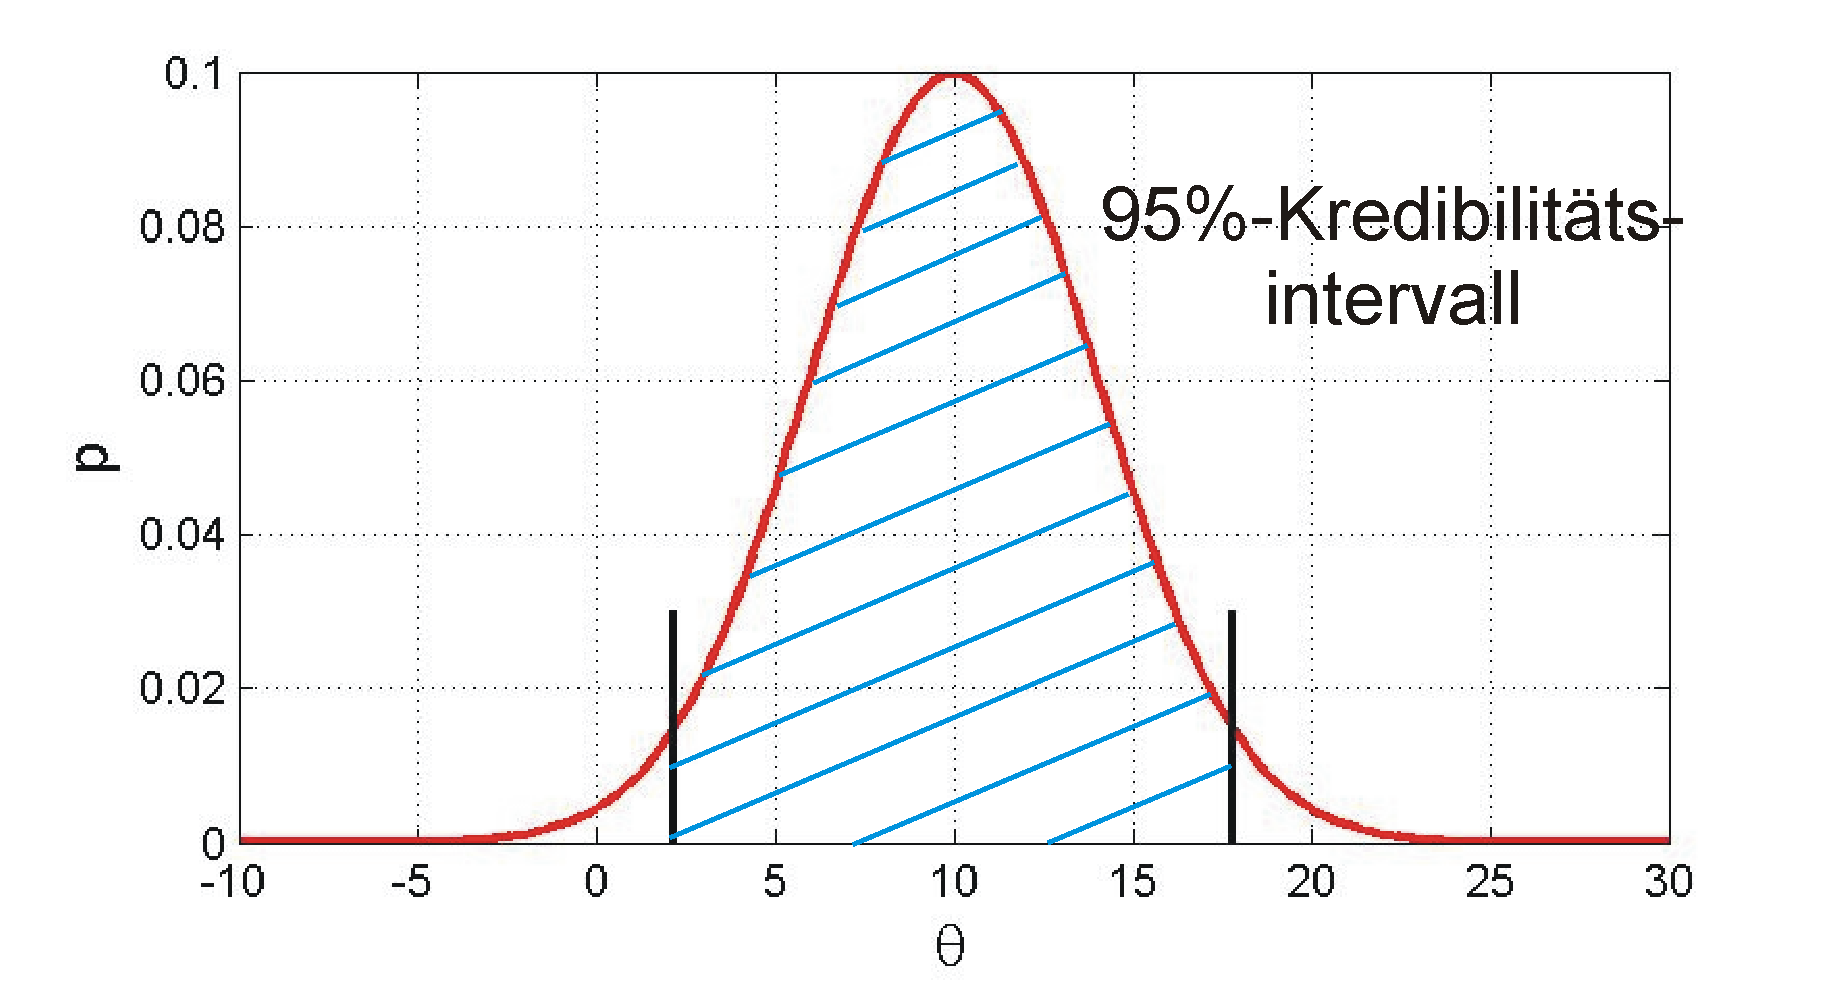
\includegraphics[width=120mm]
		{08_vorlesung/media/Posterior_Vertrauensintervall_all.png}
		\caption{Bestimmung des Kredibilitätsintervalls der Posterior-Verteilung $N(10,4^2)$für das Niveau
			$\gamma = 0.95 $, untere Grenze: $\theta_{uG}$ = 2.16, 
	    	obere Grenze $\theta_{oG}$ = 17.84}
    	\label{fig:Beispiel_Bestimmung_CredibleIntervall} 
	\end{center}
\end{figure}
(Hinweis: beidseitiges Quantil: 95\%, einseitiges Quantil 97.5\%: )

In einer Quantiltabelle der Normalverteilung (siehe z.B. im Anhang) kann der Wert 1.96 abgelesen werden.
Wir erhalten damit: 
\[
\frac{\theta_{oG}-10}{4} = 1.96 \rightarrow \theta_{oG} = 17.84 
\rightarrow \theta_{uG} = 17.84 - 2 \cdot 7.84 = 2.16
\]
Bei nichtsymmetrischen Intervallen lassen sich unterschiedliche obere und untere Grenzen finden, die zum gleichen Kredibilitätsintervall gehören. Dies ist in 
Abb. \ref{fig:Beispiel_Bestimmung_CredibleIntervall_nichtsymmetrisch}
schematisch in dem Beispiel mit der $\mathcal{X}^2$-Verteilung mit $N=10$ Freiheitsgraden dargestellt.

\begin{figure}[!htb]
	\begin{center}
		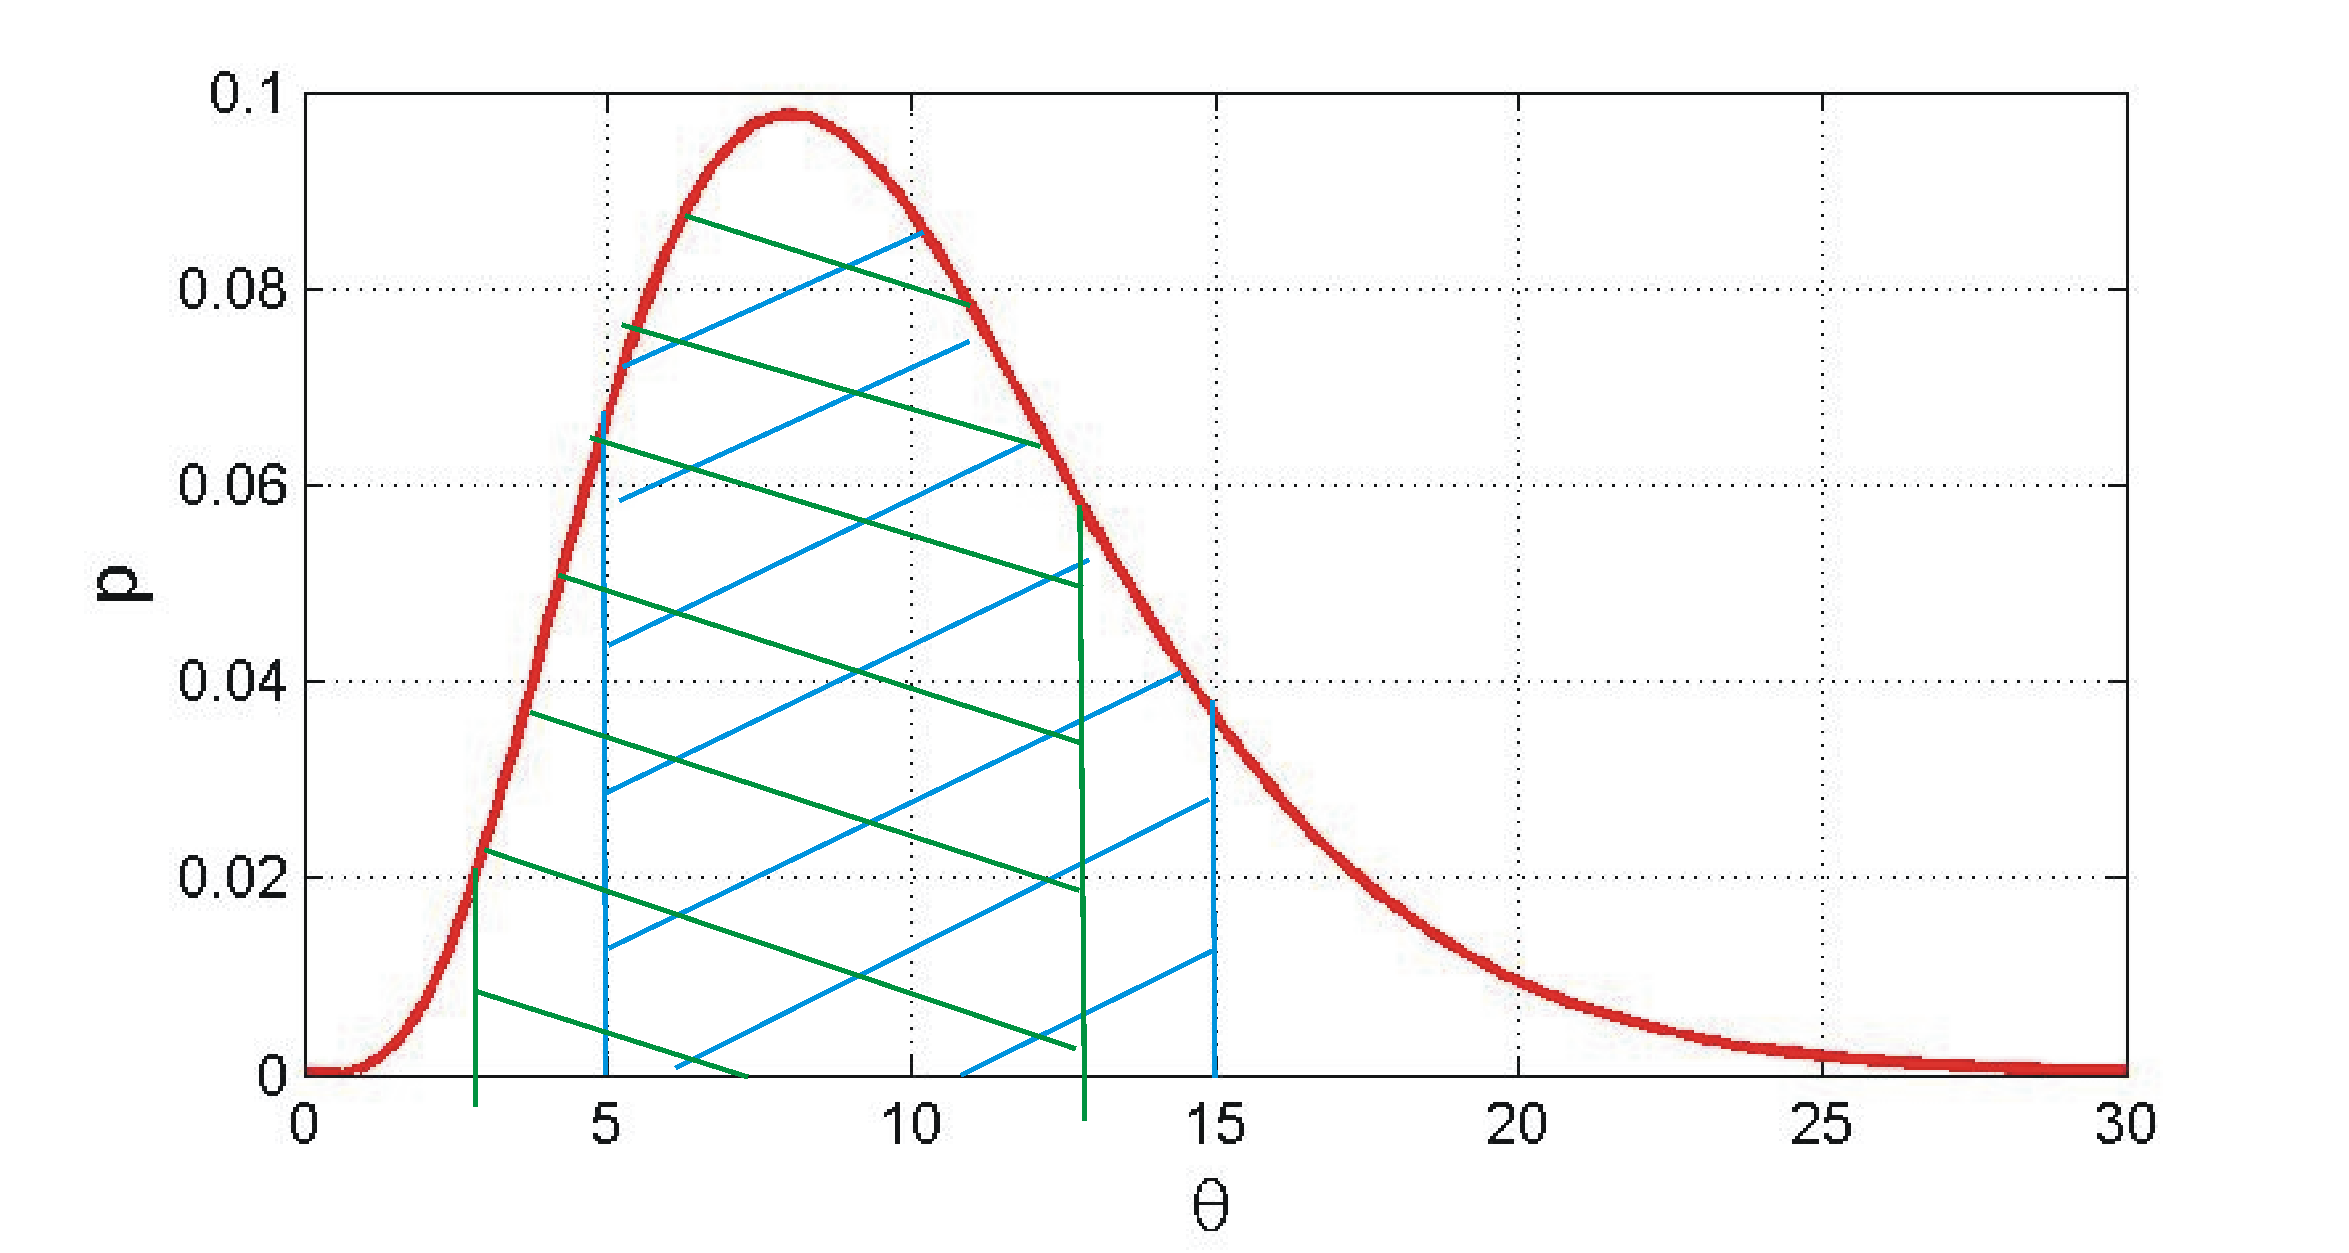
\includegraphics[width=120mm]
		{08_vorlesung/media/Posterior_Vertrauensintervall_Chi2_all.png}
		\caption{
			Bestimmung des Credible-Intervalls einer $\mathcal{X}^2$-Verteilung für 
		$N=10$ Freiheitsgrade. Der grün und blau schraffierte Bereich hat 
	dasselbe Kredibilitätsniveau.}
     \label{fig:Beispiel_Bestimmung_CredibleIntervall_nichtsymmetrisch} 
	\end{center}
\end{figure}
\subsection{MU-Bestimmung mit der Bayesschen Statisktik}
In der 9.Vorlesung werden wir den ISO-Guide 1995/2008 \cite{GUM95} noch näher kennenlernen. Er basiert im Wesentlichen auf der klassischen Statistik und hat 
folgende Einschränkungen: 
\begin{itemize}\item Der ISO Guide verwendet keine Informationen über 
	Wahrscheinlichkeitsverteilungen, die eventuell ja vorhanden
	sind. Es werden nur die Unsicherheiten fortgepflanzt jedoch keine Wahrscheinlichkeitsverteilungen.
	\item Das Messergebnis gibt keine vollständige Information wieder, da keine Wahrscheinlichkeitsverteilung angegeben wird.
	\item Die Fehlerfortpflanzung erfordert Sensitivitäten.
\end{itemize}
Der ISO-Guide ist dennoch heutzutage der Leitfaden zur Angabe der 
Messunsicherheit z.B. für Angabe der Messunsicherheit auf Kalibrierscheinen.
Wenn die pdf der Messgröße $Y$ normalverteilt ist, hat das Überdeckungsintervall
$[y\pm 2 u(y)]$ eine Überdeckungswahrscheinlichkeit von 95.45\% (siehe Tabelle G.2 im ISO-Guide \cite{GUM95}).
Bei anderen Verteilungen kann die Überdeckungswahrscheinlichkeit $p$ des Intervalls $[y \pm 2 u(y)]$ kleiner oder 
größer sein. Der ISO-Guide (Abschnitt 2.3.5 und 6.3.2) schreibt, dass ohne 
Kenntnis der Verteilung auch keine Überdeckungswahrscheinlichkeiten bestimmt werden können. Schlussendlich schlägt der ISO-Guide jedoch dann vor, dass für die 
Messgröße $Y$ eine Normalverteilung oder eine skalierte und 
geschiftete Normalverteilung angenommen werden soll.
Es wird dann vorgschlagen, dass die erweiterte Messunsicherheit 
$U_p=k_p u_c(y)$ ($u_c$: Kombinierte Standardunsicherheit) für ein Grad des Vertrauens $p$ (siehe Guide G 6.4) mit 
Hilfe der Welch-Satterthwaite Formel berechnet werden soll. Diese Formel
bietet eine Näherung bei gemischten Verteilungen der Messgrößen $X_i$
(siehe 7. Vorlesung).

In der Bayesschen Statisitk wird die Standard-Unsicherheit vom Typ-A-Fehler nicht mehr als ein Schätzwert sondern als ein Parameter des Kenntnisstandes der pdf betrachtet.
Es wird auch das Konzept der effektiven Freiheitsgrade nicht mehr benötigt.
Die Typ-A-Unsicherheit wird anders ausgewertet. Es ergibt sich für die Standardunsicherheit $u(x_i) = \sqrt{(n-1)/(n-3)} \cdot s_i/\sqrt{n}$ \cite{Kac03}. 


Den aktuellen Leitfaden ISO-Guide komplett auf die Bayes-Statistik umzuschreiben und für alle (z.B auch Kalibrierlaboratorien) verpflichtend einzuführen, fand keine Mehrheit.  
Dennoch ist es in vielen Fällen sinnvoller und richtiger die 
Messunsicherheitsbestimmung mit der Bayes-Statistik durchzuführen. Ziel der Bayesschen Statsistik ist es die PDF (probability density function) $p(Y|X)$ der Messgröße $Y$ 
zu bestimmen. Bestimmt man davon den Erwartungwert $y$, erhält man den besten Schätzwert für die Messgröße. Die Standardabweichung von $Y$ ergibt die 
zugeordnete Standardunsicherheit $u(y)$. Das Überdeckungsintervall (engl.\ \textsl{coverage integral}) wird dann aus der Posterior $p(Y|X)$ bestimmt.
Der Erwartungswert der Posterior ist der beste Schätzer für die Messgröße Y: 
\[
E(Y) = y = \int_{-\infty}^{\infty} Y \; p(Y|X) \; dY
\]
Die Varianz ist ein Maß für die Messunsicherheit: 
\begin{align}
u^2(y) =: \operatorname{Var}(Y) =& E \left( (y -E(Y)^2\right) \\[2ex]
 =&  \int\limits_{-\infty}^{\infty} (y-Y)^2 \cdot p(Y|X) dY 
\end{align}
Zur Bestimmung der Posterior kann wiederum das Bayes-Theorem angewendet werden.
\begin{equation}
p(Y|X) \propto l(Y|X) \cdot p(Y)
\end{equation}
Anstelle der Likelihood $l(Y|X)$ wird häufig die bedingte Wahrscheinlichkeitsdichte 
$p(X|Y)$ geschrieben. 
\[
p(Y|X) \propto p(X|Y) \cdot p(Y)
\]
Wir bezeichnen $p(Y)$ als die Prior-Wahrscheinlichkeit, 
$l(Y|X)$ Likelihood der Messdaten bzw. $p(X|Y)$ die Wahrscheinlichkeitsdichte 
der Messdaten und $p(Y|X)$ die gesuchte Posterior-Wahrscheinlichkeitsdichte. 
Oftmals ist es nicht möglich die Integrale analytisch zu lösen und es kommen 
numerische Integrationsmethoden zum Einsatz. Bei komplexen Modellen mit vielen
Parametern sind numerische Verfahren mit gleichförmigem Raster zu kostspielig /langwierig.  Für solche Fälle werden statistische Integrationsmethoden eingesetzt, bei denen die Positionen, an denen die zu integrierende Funktion auszurechnen ist, gewürfelt werden. Solche Methoden nennt man wegen des Auswürfelns, also des Verwendens von Pseudozufallszahlen, in Erinnerung an Spielcasinos Monte-Carlo-Methoden. Es gibt dazu unterschiedliche Strategien wie beispielsweise das Markov-Ketten-Monte-Carlo.

\section{Regression mit Vorkenntnis (Prior)}
Wir hatten klassisch die Regressionsrechnung nach der Methode der kleinsten Quadrate
(\textsl{Least Squares}) berechnet, also
$$
\min\limits_{\theta} \left\{ \left(
\mathbf{Y}^\mathsf{T}
\; - \; 
\boldsymbol{\theta}^\mathsf{T} \mathbf{X}^\mathsf{T} \right)
\left( \mathbf{Y} \; - \;  \mathbf{X} \boldsymbol{\theta} \right)\right\}
$$
was äquivalent dem Maximieren der Likelihood ist
\begin{equation}
\max\limits_{\theta} \left\{ e^{-\frac{1}{2 \, \sigma_{\varepsilon}^2} \left(
	\mathbf{Y}^\mathsf{T}
	\; - \; 
	\boldsymbol{\theta}^\mathsf{T} \mathbf{X}^\mathsf{T} \right)
	\left(\mathbf{Y} \; - \;  \mathbf{X} \boldsymbol{\theta} \right)} \right\} .
\end{equation}

Wir stellen uns vor, dass von einer vorherigen Messkampagne $\kappa-1$ zu der gleichen Messaufgabe
für alle Regressionparameter $\hat \theta_l^{(\kappa-1)}$ mit $l = 1,\dots,M$ schon ein vollständiges Messergebnis mit
\begin{equation}
\arraycolsep=2.0pt\def\arraystretch{2.0}
\begin{array}{ll}
\hat \theta_l^{(\kappa-1)} \; = \; \boldsymbol{e}_l^\mathsf{T} \, \boldsymbol{\hat \theta}^{(\kappa-1)} \; = \; &
\boldsymbol{e}_l^\mathsf{T} \, \left( \left(\mathbf{X}^{(\kappa-1)}\right)^\mathsf{T}  \, \mathbf{X}^{(\kappa-1)} \right)^{-1} \left(\mathbf{X}^{(\kappa-1)}\right) \, \mathbf{Y}^{(\kappa-1)} \\
& \; \pm \; t_{1-\alpha/2, \nu^{(\kappa-1)}} \,
\boldsymbol{e}_l^\mathsf{T} \,  \left( \left(\mathbf{X}^{(\kappa-1)}\right)^\mathsf{T} \, \mathbf{X}^{(\kappa-1)} \right)^{-1}  \boldsymbol{e}_l \, 
\, \left(\hat \sigma_{\varepsilon}^{(\kappa-1)}\right)^2
\end{array}
\end{equation}
und
\begin{equation}
\rho_{l,m} \; = \;
\frac{\left(\hat \sigma_{\varepsilon}^{(\kappa-1)}\right)^2}{\hat \sigma_l^{(\kappa-1)} \,
	\hat \sigma_m^{(\kappa-1)}} \; \boldsymbol{e}_l^\mathsf{T} \,
\left( \left(\mathbf{X}^{(\kappa-1)}\right)^\mathsf{T} \, \mathbf{X}^{(\kappa-1)} \right)^{-1} \, \boldsymbol{e}_m 
\end{equation}
vorliegt, das wir mit neuen Informationen aus
unserer neuen Messkampagne $\kappa$ \textsl{updaten} wollen.

Die Likelihood mit den Beobachtungen unserer aktuellen Kampagne ist
\begin{equation}
l(\boldsymbol{\theta}, \sigma_{\varepsilon} | \mathbf{Y}^{(\kappa)}) \; \propto \;
e^{-\frac{1}{2 \, \sigma_{\varepsilon}^2}
	\left(\mathbf{Y}^{(\kappa)} \; - \;  \mathbf{X}^{(\kappa)} \boldsymbol{\theta} \right)^\mathsf{T}
	\left(\mathbf{Y}^{(\kappa)} \; - \;  \mathbf{X}^{(\kappa)} \boldsymbol{\theta} \right)}
\end{equation}
wobei die Regressanden $\mathbf{Y}^{(\kappa)}$ mit $\sigma_{\varepsilon}$ streuen, nicht
aber die Regressoren $\mathbf{X}^{(\kappa)}$ und wobei die Modellparameter
$\boldsymbol{\theta}$ und $\sigma_{\varepsilon}$ die zu schätzenden Größen sind.

Die Wahrscheinlichkeitsdichteverteilung der vorherigen Messkampagne $\kappa-1$
ist
\begin{equation}
p_{\kappa-1}(\boldsymbol{\theta} | \boldsymbol{\hat \theta}^{(\kappa-1)}, 
\boldsymbol{\hat \Sigma}^{(\kappa-1)}_{\boldsymbol{\theta}})
\; \propto \; e^{-\frac{1}{2} 
	\left(\boldsymbol{\theta} - \boldsymbol{\hat \theta}^{(\kappa-1)} \right)^\mathsf{T} \,
	\left(\boldsymbol{\hat \Sigma}_{\boldsymbol{\theta}}^{(\kappa-1)}\right)^{-1} \, \left(\boldsymbol{\theta} - \boldsymbol{\hat \theta}^{(\kappa-1)} \right)}
\label{priorRegression}
\end{equation}
mit
$$
\boldsymbol{\hat \Sigma}_{\boldsymbol{\theta}}^{(\kappa-1)} \; = \; 
\left( \left(\mathbf{X}^{(\kappa-1)}\right)^\mathsf{T} \, \mathbf{X}^{(\kappa-1)} \right)^{-1} 
\, \left(\hat \sigma_{\varepsilon}^{(\kappa-1)}\right)^2 .
$$
Die Likelihood wird im folgenden formal so aufgeschrieben, dass zu lesen ist, dass es die
Wahrscheinlichkeitsdichteverteilung des Regressanden ist, gegeben die Parameter
$\boldsymbol{\theta}$ und $\sigma_{\varepsilon}$
\begin{equation}
p_{\mathrm{L},\kappa} (\mathbf{Y}^{(\kappa)} | \boldsymbol{\theta}, \sigma_{\varepsilon}) \; \propto \;
e^{-\frac{1}{2 \, \sigma_{\varepsilon}^2}
	\left(\mathbf{Y}^{(\kappa)} \; - \;  \mathbf{X}^{(\kappa)} \boldsymbol{\theta} \right)^\mathsf{T}
	\left(\mathbf{Y}^{(\kappa)} \; - \;  \mathbf{X}^{(\kappa)} \boldsymbol{\theta} \right)} .
\end{equation}
Wir sehen, dass dies an der Verteilung selber hier nichts verändert, sondern nur der
Interpretation dient, ob man auf die Verteilung des Regressanden (der direkten
Messgröße) guckt oder auf die Verteilung der Modellparameter (der indirekten Messgrößen).
% https://en.wikipedia.org/wiki/Naive_Bayes_classifier

Zur Schätzung der Modellparameter $\boldsymbol{\theta}$ und $\sigma_{\varepsilon}$
berechnen wir die Wahrscheinlichkeitsdichteverteilung als Funktion von
$\boldsymbol{\theta}$ und $\sigma_{\varepsilon}$.

Bei der Methode der kleinsten Quadrate fiel das $\sigma_{\varepsilon}$ zunächst raus,
so dass der Schätzvorgang nur für das $\boldsymbol{\theta}$ durchzuführen war und nach
Erhalt der Schätzer $\boldsymbol{\hat \theta}$ für die Modellparameter
$\boldsymbol{\theta}$ die entsprechende empirische Standardabweichung
$\hat \sigma_{\varepsilon}$ ausgerechnet wurde.

Dass für die Likelihood und für die Verteilungsdichte der Parameter der
vorherigen Messkampagne $\kappa-1$ Normalverteilungen angesetzt wurden, bedeutet folgendes:
Als {\`a} priori-Information wurde in das Modell die Voraussetzung hineingesteckt, dass
\begin{equation}
Y_j \, \sim \, \mathcal{N}(\boldsymbol{\theta}^\mathsf{T} \left(
\begin{array}{c} 1\\ X_{1,j}\\ \vdots \\ X_{M-1,j}\end{array}\right), \sigma_{\varepsilon})
\qquad \Leftrightarrow \qquad
\varepsilon_j \, \sim \, \mathcal{N}(0, \sigma_{\varepsilon})
\end{equation}
und
\begin{equation}
\boldsymbol{\theta}^{(\kappa-1)} \, \sim \, 
\mathcal{N}(\boldsymbol{\hat \theta}^{(\kappa-1)}, 
\boldsymbol{\hat \Sigma}_{\boldsymbol{\theta}}^{(\kappa-1)}) .
\end{equation}
Für das $\sigma_{\varepsilon}$ setzen wir voraus, dass es $\chi^2$-verteilt sei
\begin{equation}
\nu \left(\frac{\sigma_{\varepsilon}}{\hat \sigma_{\varepsilon}^{(\kappa,\mathrm{R})}}\right)^2
\; \sim \; \chi^2_{\nu}
\end{equation}
wobei wir für $\hat \sigma_{\varepsilon}^{(\kappa,\mathrm{R})}$ beispielsweise das Ergebnis
für die lineare Regression ohne Berücksichtigung der vorherigen Messkampagne, also gemäß
der im vorigen Kapitel beschriebenen Methode, verwenden.
% p_{\chi^2} (\hat \sigma_{\varepsilon}^{(\kappa,\mathrm{R})}, \nu)

Als Prior-Verteilungen haben wir nun zum einen die Verteilung aus der 
Erfahrung der vorherigen Messkampagne(n) $\kappa-1$, Gl.~(\ref{priorRegression})
und zum anderen die Verteilung für $\sigma_{\varepsilon}$
\begin{equation}
p_{\chi^2} (\sigma_{\varepsilon} | \hat \sigma_{\varepsilon}^{(\kappa,\mathrm{R})}, \nu) .
\label{priorSigmaEpsi}
\end{equation}

Die Posterior-Verteilung ist damit
\begin{equation}
\arraycolsep=2.0pt\def\arraystretch{2.0}
\begin{array}{l}
p_{\kappa}(\boldsymbol{\theta}, \boldsymbol{\Sigma}_{\boldsymbol{\theta}} | \mathbf{Y}^{(\kappa)}, \hat \sigma_{\varepsilon}^{(\kappa,\mathrm{R})},  \boldsymbol{\hat \theta}^{(\kappa-1)},  \boldsymbol{\hat \Sigma}^{(\kappa-1)}_{\boldsymbol{\theta}}) \\
\propto
\; p_{\mathrm{L},\kappa} (\mathbf{Y}^{(\kappa)} | \boldsymbol{\theta}, \sigma_{\varepsilon}) \,
p_{\chi^2} (\sigma_{\varepsilon} | \hat \sigma_{\varepsilon}^{(\kappa,\mathrm{R})}, \nu) \,
p_{\kappa-1}(\boldsymbol{\theta} | \boldsymbol{\hat \theta}^{(\kappa-1)}, 
\boldsymbol{\hat \Sigma}^{(\kappa-1)}_{\boldsymbol{\theta}})  .
\end{array}
\end{equation}
Da in den $\mathbf{Y}^{(\kappa)}$ nur die Regressoren und die $\sigma_{\varepsilon}$ stecken
$$
\boldsymbol{\Sigma}_{\boldsymbol{\theta}} \; = \;
\left( \left(\mathbf{X}^{(\kappa)}\right)^\mathsf{T} \, \mathbf{X}^{(\kappa)} \right)^{-1} 
\sigma_{\varepsilon}^2 
$$
brauchen wir nicht das gesamte $\boldsymbol{\Sigma}_{\boldsymbol{\theta}}$ als Funktionsvariable,
sondern lediglich $\sigma_{\varepsilon}$, so dass die Posterior nur noch
Funktion von $\boldsymbol{\theta}$ und $\sigma_{\varepsilon}$ ist
\begin{equation}
\arraycolsep=2.0pt\def\arraystretch{2.0}
\begin{array}{l}
p_{\kappa}(\boldsymbol{\theta}, \sigma_{\varepsilon} | \mathbf{Y}^{(\kappa)}, \hat \sigma_{\varepsilon}^{(\kappa,\mathrm{R})},  \boldsymbol{\hat \theta}^{(\kappa-1)},  \boldsymbol{\hat \Sigma}^{(\kappa-1)}_{\boldsymbol{\theta}}) \\
\propto
\; p_{\mathrm{L},\kappa} (\mathbf{Y}^{(\kappa)} | \boldsymbol{\theta}, \sigma_{\varepsilon}) \,
p_{\chi^2} (\sigma_{\varepsilon} | \hat \sigma_{\varepsilon}^{(\kappa,\mathrm{R})}, \nu) \,
p_{\kappa-1}(\boldsymbol{\theta} | \boldsymbol{\hat \theta}^{(\kappa-1)}, 
\boldsymbol{\hat \Sigma}^{(\kappa-1)}_{\boldsymbol{\theta}})  .
\end{array}
\label{posteriorRegression}
\end{equation}
Für das vollständige Messergebnis berechnen wir die Marginalverteilung als Funktion von
$\boldsymbol{\theta}$, indem wir über $\sigma_{\varepsilon}$ integrieren
\begin{equation}
p_{\kappa}(\boldsymbol{\theta}| \mathbf{Y}^{(\kappa)}, \hat \sigma_{\varepsilon}^{(\kappa,\mathrm{R})},  \boldsymbol{\hat \theta}^{(\kappa-1)},  \boldsymbol{\hat \Sigma}^{(\kappa-1)}_{\boldsymbol{\theta}}) \; = \; 
\int\limits_0^\infty \, p_{\kappa}(\boldsymbol{\theta}, \sigma_{\varepsilon} | \mathbf{Y}^{(\kappa)}, \hat \sigma_{\varepsilon}^{(\kappa,\mathrm{R})},  \boldsymbol{\hat \theta}^{(\kappa-1)},  \boldsymbol{\hat \Sigma}^{(\kappa-1)}_{\boldsymbol{\theta}}) \;
\operatorname{d}\sigma_{\varepsilon} .
\end{equation}

Dies ist eine Funktion von $M$ Variablen $\theta_1, \dots, \theta_M$.
Für die Wahrscheinlichkeitsdichten als Marginalverteilung je eines der
Regressionsparameter wird über die anderen (numerisch) integriert
\begin{equation}
\arraycolsep=2.0pt\def\arraystretch{2.0}
\begin{array}{l}
p_{\kappa}(\theta_m | \mathbf{Y}^{(\kappa)}, \hat \sigma_{\varepsilon}^{(\kappa,\mathrm{R})},  \boldsymbol{\hat \theta}^{(\kappa-1)},  \boldsymbol{\hat \Sigma}^{(\kappa-1)}_{\boldsymbol{\theta}}) \;
\; =\\
\int\limits_{-\infty}^\infty \dots \int\limits_{-\infty}^\infty
p_{\kappa}(\boldsymbol{\theta}| \mathbf{Y}^{(\kappa)}, \hat \sigma_{\varepsilon}^{(\kappa,\mathrm{R})},  \boldsymbol{\hat \theta}^{(\kappa-1)},  \boldsymbol{\hat \Sigma}^{(\kappa-1)}_{\boldsymbol{\theta}}) \operatorname{d}\theta_1 \dots \operatorname{d}\theta_{m-1} \, \operatorname{d}\theta_{m+1} \dots
\operatorname{d}\theta_M .
\end{array}
\end{equation}
Zur Berechnung der Erwartungswertes wird (numerisch) integriert
\begin{equation}
\operatorname{E}(\theta_m) \; = \;
\int\limits_{-\infty}^\infty \; \theta_m \;
p_{\kappa}(\theta_m | \mathbf{Y}^{(\kappa)}, \hat \sigma_{\varepsilon}^{(\kappa,\mathrm{R})},  \boldsymbol{\hat \theta}^{(\kappa-1)},  \boldsymbol{\hat \Sigma}^{(\kappa-1)}_{\boldsymbol{\theta}}) \;
\operatorname{d}\theta_{m} .
\end{equation}
Das \textsl{Credible Interval} wird ebenso mittels numerischer Verfahren berechnet
\begin{equation}
\alpha/2 \; = \; \int\limits_{-\infty}^{\theta_{m,\mathrm{min}}} \; p_{\kappa}(\theta_m | \mathbf{Y}^{(\kappa)}, \hat \sigma_{\varepsilon}^{(\kappa,\mathrm{R})},  \boldsymbol{\hat \theta}^{(\kappa-1)},  \boldsymbol{\hat \Sigma}^{(\kappa-1)}_{\boldsymbol{\theta}}) \;
\operatorname{d}\theta_{m}
\end{equation}
und
\begin{equation}
1 - \alpha/2 \; = \; \int\limits_{-\infty}^{\theta_{m,\mathrm{max}}} \; p_{\kappa}(\theta_m | \mathbf{Y}^{(\kappa)}, \hat \sigma_{\varepsilon}^{(\kappa,\mathrm{R})},  \boldsymbol{\hat \theta}^{(\kappa-1)},  \boldsymbol{\hat \Sigma}^{(\kappa-1)}_{\boldsymbol{\theta}}) \;
\operatorname{d}\theta_{m} .
\end{equation}

Für die Regressionsanalyse kann auch eine Möglichkeit gefunden werden, eine analytische
Lösung zu erhalten, wenn anstelle der $\chi^2$-Verteilung für die $\sigma_{\varepsilon}$
eine Verteilung gewählt wird, so dass sich das Produkt aus Likelihood und einer
alternativen Verteilung $p_{\mathrm{a}}(\sigma_{\varepsilon})$
vereinfachen lässt, wie es in Klauenberg \textsl{et al.\ } dargelegt wird \cite{Kla15}.

Da $p_{\kappa-1}$ nicht von $\sigma_{\varepsilon}$ abhängt, gilt
\begin{equation}
\arraycolsep=2.0pt\def\arraystretch{2.0}
\begin{array}{l}
p_{\kappa}(\boldsymbol{\theta}| \mathbf{Y}^{(\kappa)}, \hat \sigma_{\varepsilon}^{(\kappa,\mathrm{R})},  \boldsymbol{\hat \theta}^{(\kappa-1)},  \boldsymbol{\hat \Sigma}^{(\kappa-1)}_{\boldsymbol{\theta}}) \\
\; \propto \; p_{\kappa-1}(\boldsymbol{\theta} | \boldsymbol{\hat \theta}^{(\kappa-1)}, 
\boldsymbol{\hat \Sigma}^{(\kappa-1)}_{\boldsymbol{\theta}}) \, 
\int\limits_0^\infty \, p_{\mathrm{L},\kappa} (\mathbf{Y}^{(\kappa)} | \boldsymbol{\theta},
\sigma_{\varepsilon}) \;
p_{\mathrm{a}} (\sigma_{\varepsilon} | \hat \sigma_{\varepsilon}^{(\kappa,\mathrm{R})}, \nu) \;
\operatorname{d}\sigma_{\varepsilon}
\end{array}
\end{equation}
und mit einer vereinfachten Verteilung $p_{\mathrm{a}}(\sigma_{\varepsilon})$
\begin{equation}
\int\limits_0^\infty \, p_{\mathrm{L},\kappa} (\mathbf{Y}^{(\kappa)} |
\boldsymbol{\theta}, \sigma_{\varepsilon}) \;
p_{\mathrm{a}} (\sigma_{\varepsilon} | \hat \sigma_{\varepsilon}^{(\kappa,\mathrm{R})}, \nu) \;
\operatorname{d}\sigma_{\varepsilon}
\; \propto \;
e^{- \frac{1}{2} \, \left(\frac{f(\nu)}{\hat \sigma_{\varepsilon}^{(\kappa,\mathrm{R})}}\right)^2
	\left(\mathbf{Y}^{(\kappa)} \; - \;  \mathbf{X}^{(\kappa)} \boldsymbol{\theta} \right)^\mathsf{T}
	\left(\mathbf{Y}^{(\kappa)} \; - \;  \mathbf{X}^{(\kappa)} \boldsymbol{\theta} \right)}
\end{equation}
mit $f(\nu)$ eine sich aus $p_{\mathrm{a}}$ ergebende Funktion der Anzahl der Freiheitsgrade.

Mit Gl.~(\ref{priorRegression}) bekommen wir
\begin{equation}
\arraycolsep=2.0pt\def\arraystretch{2.0}
\begin{array}{l}
p_{\kappa}(\boldsymbol{\theta}| \mathbf{Y}^{(\kappa)}, \hat \sigma_{\varepsilon}^{(\kappa,\mathrm{R})},  \boldsymbol{\hat \theta}^{(\kappa-1)},  \boldsymbol{\hat \Sigma}^{(\kappa-1)}_{\boldsymbol{\theta}}) \; \propto \\
e^{-\frac{1}{2} 
	\left(\boldsymbol{\theta} - \boldsymbol{\hat \theta}^{(\kappa-1)} \right)^\mathsf{T} \,
	\left(\boldsymbol{\hat \Sigma}_{\boldsymbol{\theta}}^{(\kappa-1)}\right)^{-1} \, \left(\boldsymbol{\theta} - \boldsymbol{\hat \theta}^{(\kappa-1)} \right)} \;
e^{- \frac{1}{2} \, \left(\frac{f(\nu)}{\hat \sigma_{\varepsilon}^{(\kappa,\mathrm{R})}}\right)^2
	\left(\mathbf{Y}^{(\kappa)} \; - \;  \mathbf{X}^{(\kappa)} \boldsymbol{\theta} \right)^\mathsf{T}
	\left(\mathbf{Y}^{(\kappa)} \; - \;  \mathbf{X}^{(\kappa)} \boldsymbol{\theta} \right)}
\end{array}
\end{equation}
so dass die Schätzer für $\boldsymbol{\theta}$ und $\boldsymbol{\Sigma}_{\boldsymbol{\theta}}$
wie folgt aussehen
\begin{equation}
\arraycolsep=2.0pt\def\arraystretch{2.0}
\begin{array}{l}
\boldsymbol{\hat \theta}^{(\kappa)} \; = \; \\
\left(
\left(\frac{\hat \sigma_{\varepsilon}^{(\kappa,\mathrm{R})}}{f(\nu)}\right)^2 \,
\left(\boldsymbol{\hat \Sigma}_{\boldsymbol{\theta}}^{(\kappa-1)}\right)^{-1}
\; + \;
\left(\mathbf{X}^{(\kappa)}\right)^\mathsf{T} \, \mathbf{X}^{(\kappa)} 
\right)^{-1} \;
\left(
\left( \frac{\hat \sigma_{\varepsilon}^{(\kappa,\mathrm{R})}}{f(\nu)}\right)^2 \,
\left(\boldsymbol{\hat \Sigma}_{\boldsymbol{\theta}}^{(\kappa-1)}\right)^{-1} \,
\boldsymbol{\theta}^{(\kappa-1)} \; + \;
\left(\mathbf{X}^{(\kappa)}\right)^\mathsf{T} \, \mathbf{Y}^{(\kappa)} \right)
\end{array}
\end{equation}
und
\begin{equation}
\boldsymbol{\hat \Sigma}_{\boldsymbol{\theta}}^{(\kappa)} \; = \;
\left(
\left(\boldsymbol{\hat \Sigma}_{\boldsymbol{\theta}}^{(\kappa-1)}\right)^{-1}
\; + \;
\left(\mathbf{X}^{(\kappa)}\right)^\mathsf{T} \, \mathbf{X}^{(\kappa)}  \,
\left(\frac{f(\nu)}{\hat \sigma_{\varepsilon}^{(\kappa,\mathrm{R})}}\right)^2
\right)^{-1} 
\end{equation}
siehe auch das von K. Klauenberg mitverfasste Tutorial \cite{Els15}, das ausführlicher
in der Beschreibung ist als ihre Publikation \cite{Kla15} und auch 
beispielhaft Matlab-Skripte enthält.

\section{Median einer Verteilung}
Wir haben bisher den Erwartungswert einer Verteilung (1. statistisches Moment) und höhere Momente von Verteilungen (Varianz, Skewness, Kurtosis) kennengelernt, siehe 5. Vorlesung. Unter den symmetrischen Verteilungen unterscheiden wir: 
\begin{itemize}
	\item die Normalverteilung,
	\item die t-Verteilung, deren Ausläufer (\textit{Tails}) um so ausgeprägter sind je kleiner die Anzahl der Freiheitsgrade ist, 
	\item die Laplace-Verteilungen, die sehr lange Ausläufer hat. Sie 
	setzt sich aus zwei aneinandergefügten Exponentialverteilungen zusammen, siehe
	3. Vorlesung Gl.(3.6).  
\end{itemize}

Für die Schätzung eines Modellparameters $\theta$ haben wir in 
der 1. und 2. Vorlesung die Methode der Maximum Likelihood kenengelernt 
(\glqq Finde den Parameter $\theta$, sodass die Likelihood maximal wird\grqq). Diese Methode führt bei normalverteilten Größen zum Least Square (Minimierung der Residuen) und wird als \textit{L2-Norm} bezeichnet. 

Zuvor hatten wir gesehen wie die Maximierung der Likelihood
$l(\theta) \propto e^{-\frac{1}{2}\sum_i \left(\frac{\varepsilon_i(\theta)}{\sigma}\right)^2}$
in die Minimierung der Summe der Quadrate der Residuen übergeht
$$
\max_{\theta} \left\{ e^{-\frac{1}{2}\sum_i \left(\frac{\varepsilon_i(\theta)}{\sigma}\right)^2} \right\}
\quad \Rightarrow \quad
\min_{\theta} \left\{ -\log\left(e^{-\frac{1}{2}\sum_i \left(\frac{\varepsilon_i(\theta)}{\sigma}\right)^2} \right) \right\} ,
$$
d.h.
$$
\min_{\theta} \left\{ \sum_i \left(\frac{\varepsilon_i(\theta)}{\sigma}\right)^2 \right\} .
$$
Mit $\operatorname{Var}(\boldsymbol \varepsilon) = \sum_i \varepsilon_i(\theta)^2$ bedeutet dies, dass
die Varianz der Residuen minimiert wird
\begin{equation}
\min_{\theta} \left\{ \int_{-\infty}^{\infty} \operatorname{Var}(\boldsymbol \varepsilon)  \, l(\theta) \, \operatorname d \theta \right\} .
\end{equation}

Analog lässt sich auch die Varianz bezüglich der Posterior $p(\theta|X)$ für die bayes'sche Statistik minimieren:
\begin{equation}
\min_{\theta} \left\{ \int_{-\infty}^{\infty} \operatorname{Var}(\boldsymbol \varepsilon)  \, p(\theta|X) \, \operatorname d \theta \right\} .
\end{equation}
Betrachte einen skalaren Modellparameter $\theta$ mit Schätzwert $\hat \theta$ und $\varepsilon = \theta - \hat \theta$, so dass
\begin{equation}
\min_{\theta} \left\{ \int_{-\infty}^{\infty} \varepsilon^2  \, p(\theta|X) \, \operatorname d \theta \right\} .
\end{equation}
Dabei ist $\int_{-\infty}^{\infty} \varepsilon^2  \, p(\theta|X) \, \operatorname d \theta$ gleich dem Erwartungswert der 
Residuenquadrate, mit $\varepsilon = \theta - \hat \theta$
$$
\int_{-\infty}^{\infty} \varepsilon^2  \, p(\theta|X) \, \operatorname d \theta \;
= \; E( (\theta - \hat \theta)^2 )
$$

Die erste Ableitung wird zu Null gesetzt:
\begin{equation}  
\frac{\operatorname d \epsilon}{\operatorname d \hat\theta } = \frac{\operatorname d}{\operatorname d \hat\theta } \int_{-\infty}^{\infty}
(\hat\theta - \theta)^2 p(\theta|X) \operatorname d\theta = 0 
\end{equation}
\[
2 \int_{-\infty}^{\infty} (\hat\theta - \theta) p(\theta|X) \operatorname d\theta = 0
\]
Daraus folgt: 
\[
\hat\theta \int_{-\infty}^{\infty} p(\theta|X) \operatorname d\theta = \int_{-\infty}^{\infty} \theta p(\theta|X) \operatorname d \theta
\]

Das linke Integral ist auf Grund der Normierungsbedingung $\int_{-\infty}^{\infty} p(\theta|X) d\theta = 1$. Es folgt somit: 
\begin{equation}
\hat\theta = \int_{-\infty}^{\infty} \theta p(\theta|X) d \theta = E(p(\theta|X))
\end{equation}
Der Erwartungswert $E(p(\theta|X))$ der Posterior-Verteilung $p(\theta|X)$ ist derjenige Schätzwert
$\hat{\theta}$, der die Residuen minimiert. 


Zur Behandlung von Beobachtungen, die nicht rein stochastischer Natur sind, sondern durch andere, nicht weiter
modellierbare Einflüsse gegeben sind, wie z.B. mit einer größeren Wahrscheinlichkeit - als bei der Normalverteilung in den
Ausläufern, wird beispielsweise auf die Laplaceverteilung zurückgegriffen werden. Die Maximum-Likelihood-Methode für die Laplace-Transformation führt auf die Minimierung der Absolutbeträge der Residuen (siehe 2. Vorlesung),
d.h. $\sum \left|\epsilon \right| \rightarrow \min$. Man bezeichnet dies
als die \textit{L1-Norm}. Sie liefert den \textit{Median}. Er ist 
definiert als das 0.5-Quantil $Q_{0.5}$. Ein Quantil $Q_\alpha$ ist ein Lagemaß in der Statistik (siehe 5.~Vorlesung). So liegen beim 0.5-Quantil 50\% der Verteilung unterhalb und 50\% der Verteilung oberhalb des Quantils.

Wir schauen uns die Minimierung der Erwartungswert der absoluten Abweichung zwischen 
$\hat{\theta}$ und $\theta$, d.h.  
\[
\epsilon(\hat{\theta}) := E(|\hat{\theta}-\theta|)
\;\; \rightarrow \;\; min.
\]
mit 
\[
E(|\hat{\theta}-\theta|) \; = \; \int\limits_{-\infty}^{\infty} |\hat{\theta}-\theta | p(\theta|X) \operatorname d \theta 
\]
Das Minimum erhalten wir durch Differentiation $\operatorname d \epsilon / \operatorname d \hat{\theta} = 0$
\[
\begin{array}{rcl}
\frac{\T \operatorname d \epsilon}{\T \operatorname d \hat{\theta}} &=& 
\frac{\T \operatorname d}{\T \operatorname d \hat{\theta}} 
\int\limits_{-\infty}^{\infty} |\hat{\theta}-\theta | p(\theta|X) \operatorname d \theta \\[2ex]
&=&\frac{\T \operatorname d}{\T \operatorname d \hat{\theta}} \left[\int\limits_{-\infty}^{\hat{\theta}}(\hat{\theta}-\theta) p(\theta |X) \operatorname d \theta 
+\int\limits_{\hat{\theta}}^{\infty} (\theta -\hat{\theta}) p(\theta|X))d \theta
\right] = 0
\end{array}
\]
Mit der Leibnizschen Regel für Parameterintegrale leiten wir die Gleichung
ab und erhalten: 
\[
\int_{-\infty}^{\hat{\theta}} p(\theta |X) \operatorname d \theta 
- \int_{\hat{\theta}}^{\infty} p(\theta|X)) \operatorname d \theta
= 0
\]
Die Summe der beiden Integrale ist als Dichte-Integral gleich 1. 
Daraus folgt: 
\[
\int_{-\infty}^{\hat{\theta}} p(\theta |X) \operatorname d \theta 
= \int_{\hat{\theta}}^{\infty} p(\theta|X)) \operatorname d \theta
= 0.5
\]
Somit ist $\hat{\theta}$ der Median bzw. das 50-Prozent-Quantil $Q_{0.5}$.

Der Median ist robust gegenüber langen \glqq tails\grqq und kann für 
jede beliebige Posterior-Verteilung bestimmt werden. 

\begin{figure}[!htb]
	\begin{center}
	  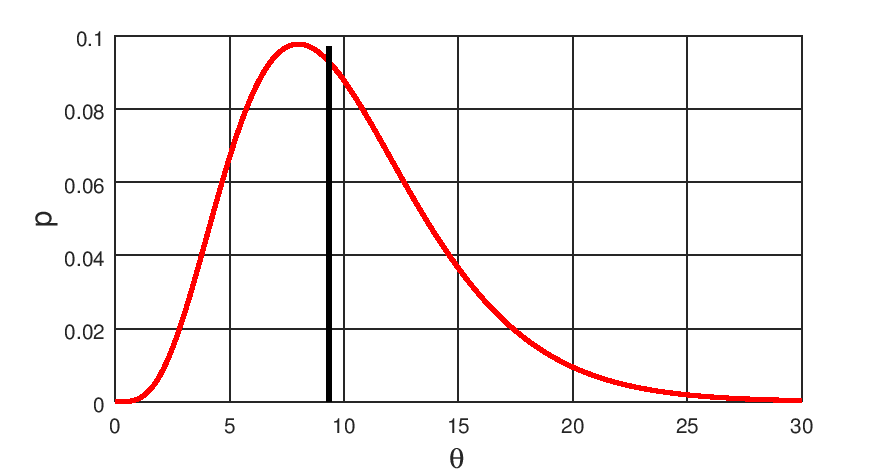
\includegraphics[width=120mm] 
		{08_vorlesung/media/Plot_Median.png}
		\caption{Beispiel für den Median, er entspricht hier nicht dem 
			Maximum. Der Median ist definiert, so dass 50 \% der Fläche unterhalb und 50 \%
		der Fläche oberhalb des Medians liegen}
	\label{fig:Median}
	\end{center}
\end{figure}

Wesentliche Unterschiede zwischen der L1-und der L2-Norm sind in 
Tab. \ref{tab:L2_und_L1_Norm} aufgezählt.
\begin{table}[!htbp]
	\caption{Unterschiede zwischen L2- und L1-Norm} 
	\vspace*{1ex}
	\label{tab:L2_und_L1_Norm}
	\centering
	\begin{tabular}{|m{8cm} | m{8cm}| }  \hline
	\textbf{L2-Norm:} & \textbf{L1-Norm:} \\
  \textbf{Minimierung der quadr. Abweichungen} & \textbf{Minimierung der Beträge} \\ \hline
   Nicht sehr robust & robust \\ \hline
   stabile Lösung & instabile Lösung möglich \\\hline
   immer nur eine Lösung möglich & mehrere Lösungen möglich \\\hline
	\end{tabular}
\end{table}


\begin{thebibliography}{------}
 \item[] \hspace*{5em}{\Large\bf zu Kapitel 8:}
\bibitem[VIM08]{VIM08} VIM International vocabulary of
metrology – Basic and general
concepts and associated terms (VIM) 3rd edition (2008)
\bibitem[GUM95]{GUM95} JCGM 100:2008 BIPM, IEC, IFCC, ISO, IUPAC, IUPAP and OIML 1995 Guide to the Expression of Uncertainty in Measurement (GUM)
(Geneva, Switzerland: International Organization for
Standardization) ISBN 92-67-10188-9
\bibitem[Kac03]{Kac03} R. Kacker, A. Jones: On use of Bayesian statistics to make the Guide to the Expression of Uncertainty in Measurement consistent, 
	Metrologia, Volume 40, Issue 5, pp. 235-248 (2003).
\bibitem[Hel08]{Hel08} L. Held: Methoden der statistischen Inferenz. 
Likelihood und Bayes. Spektrum, Heidelberg (2008)
\bibitem[Tsc14]{Tsc14} W. Tschirk: Statistik: Klassisch oder Bayes.
Zwei Wege im Vergleich, Springer Lehrbuch, (2014).
\bibitem[Kla15]{Kla15} K. Klauenberg et al. A tutorial on bayesian normal linear regression. Metrologia, 52, 2017.
\bibitem[Els15]{Els15} C. Elster, K. Klauenberg, M. Walzel, G. Wübbeler, P. Harris, M. Cox, C. Matthews, I. Smith, L. Wright, A. Allard, N. Fischer, S. Cowen, S. Ellison,
P. Wilson, F. Pennecchi, G. Kok, A. van der Veen, L. Pendrill,
A Guide to Bayesian Inference for Regression Problems, Deliverable of EMRP project NEW04 “Novel mathematical and statistical approaches to uncertainty evaluation”, 2015 \newline
www.ptb.de/emrp/fileadmin/documents/nmasatue/NEW04/Papers/BPGWP1.pdf
\end{thebibliography}

\begin{comment}
\section*{Anhang}
\begin{figure}[!h]
	\begin{center}
		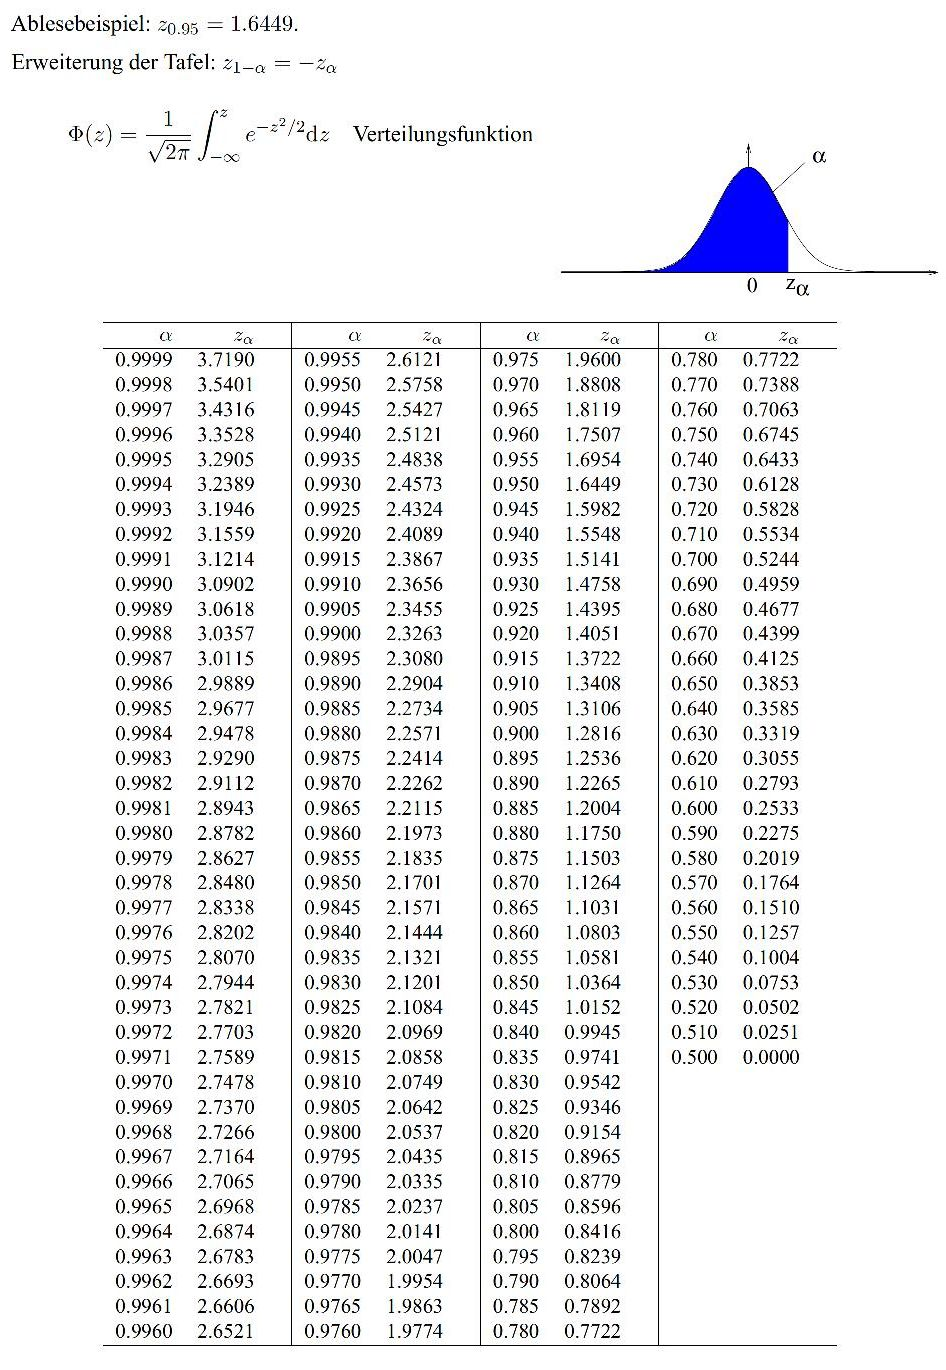
\includegraphics[width=140mm]
		{08_vorlesung/media/NV_Quantile.jpg}
		\caption{
			Quantile der Normalverteilung}
			\label{fig:Quantile_der_Normalverteilung} 
	\end{center}
\end{figure}
\end{comment}

\newpage
\section{Übungsaufgaben}
\textbf{Aufgabe 9-1: Likelihood des Erwartungswertes bei bekannter Varianz}
\begin{itemize}
	\item [(a)] Bestimmen Sie die Likelihood einer normalverteilten Zufallsgröße $X$, die sich aus $J$ unabhängigen Beobachtungen $X_1,\ldots,X_J$ ergibt. 
	Die Varianz $\sigma^2$ der Zufallsgröße $X$ sei bekannt.
\end{itemize}

\textbf{Lösung zu 9-1(a)} \\
Die Likelihoodfunktion ist gegeben durch: 
\[
l(\theta|X) = \prod_{j=1}^{J} l(\theta|X_j)
\]
Die Beobachtungen sind normalverteilt mit Erwartungswert 
$\hat{\theta}$ und Varianz $\sigma$. Es ergibt sich: 
\[
l(\theta|X) = \prod_{j=1}^{J} \frac{1}{\sqrt{(2 \pi)}} 
e^{-\;\frac{1}{2}\left(\frac{X_j-\hat{\theta}}{\sigma}\right)^2}
\]
Somit erhalten wir: 
\[
\begin{array}{rcl}
l(\theta|X) & \propto &  \prod\limits_{j=1}^{J} 
e^{-\;\frac{(X_j-\hat{\theta)}^2}{2\sigma^2}} \\[2ex]
&=& e^{-\;\frac{\T\sum\limits_{j=1}^{J}(X_j-\hat{\theta})^2}
	{\T 2 \sigma^2}} \\[2ex]
&=& e^{-\;\frac{\T\sum\limits_{j=1}^{J}(X_j^2-2X_j\hat{\theta}
	+\hat{\theta}^2)}
	{\T 2 \sigma^2}} \\[2ex]
&=& e^{-\;\frac{\T\sum\limits_{j=1}^{J}X_j^2 
		- 2 (\sum\limits_{j=1}^{J}X_j) \hat{\theta}
		+J \hat{\theta}^2}
	{\T 2 \sigma^2}} \\[2ex]
&=& e^{-\;\frac{\T \bar{X^2}-2\bar{X}\hat{\theta}+\hat{\theta}^2}
	{\T 2 \sigma^2/J}} \\[2ex]
\end{array}
\]
Die empirische Varianz $s^2$ ist gegeben durch:
\[
\begin{array}{rcl}
s^2 &=& \frac{1}{J} \sum\limits_{j=1}^{J} (X_i - \bar{X})^2 \\[2ex]
    &=& \frac{1}{J} (\sum_j X_j^2-2 \sum_j X_j \bar{X} + \sum_j \bar{X}^2) \\[2ex]
    &=& \bar{X^2} -\bar{(X)}^2 \\[2ex]
\end{array}
\] 
Damit erhalten wir für die Likelihood:
\[
\begin{array}{rcl}
l(\theta|X) & \propto & 
e^{-\;\frac{\T \bar{X}^2 +s^2 -2\bar{X} \hat{\theta}+\hat{\theta}^2}
	{\T 2 \sigma^2/J}} \\[2ex]
&=& e^{-\;\frac{\T \bar{X}^2 -2\bar{X} \hat{\theta}+\hat{\theta}^2}
	{\T 2 \sigma^2/J}}
e^{-\;\frac{\T s^2 }
	{\T 2 \sigma^2/J}} \\[2ex]
&=& e^{-\;\frac{\T (\bar{X} - \hat{\theta})^2} 
	{\T 2 \sigma^2/J}}
    \cdot e^{-\;\frac{\T s^2 }
	{\T 2 \sigma^2/J}} 
\end{array}
\]
Da der Term 
\[e^{-\;\frac{\T s^2 }
	{\T 2 \sigma^2/J}} = \mathrm{const.}
\]
ist, geht dieser Term nur in die Normierung ein. 
Es folgt für die Likelihood der Stichproben: 
\[
l(\theta|X) = l(\theta|\bar{X}) \propto e^{-\;\frac{\T (\bar{X} - \hat{\theta})^2} 
	{\T 2 \sigma^2/J}}
\]
Der Stichprobenmittelwert $\bar{X}$ ist also normalverteilt mit dem 
Erwartungwert $\hat{\theta}$ und der Varianz $\sigma^2 /J$
Hinweis / Ergänzug: Ist die Varianz von $X$ unbekannt, dann schätzen wir diese durch die empirische Varianz $s^2$ (klassische Statistik) Für annähernd große Stichproben geht die t-Verteilung in
die Normalverteilung über und der Stichprobenmittelwert ist normalverteilt mit der Varianz $s^2/J$. Dann erhalten wir analog für die Likelihood des Mittelwertes: 
\[
l(\theta|\bar{X}) \propto e^{-\;\frac{\T (\bar{X} - \hat{\theta})^2} 
	{\T 2 s^2/J}}
\]
\textbf{Aufgabe 9-2: Bestimmung des Credible-Intervalls einer Posterior-Verteilung} \\
Sie wollen die Temperatur $T$ eines Laborraumes bestimmen. 
Da hier $T$ der zu bestimmende Parameter ist, bezeichnen 
wir diesen im Folgenden mit $\theta$.
Aus Erfahrung wissen wir (wenn die Klimaanlage gerade nicht ausgefallen ist :-)), dass die Temperatur normalverteilt bei $20^{\circ}\textrm{C}$ \ 
 mit einer Steuung von $2^{\circ}\textrm{C}$ ist. D.h. als Prior nehmen wir an 
$\theta \sim N(\mu=20,\sigma^2=2^2)$. Zur genauen Bestimmung der 
Labortemperatur verwenden Sie nun einen Temperaturfühler, der einer 
Normalverteilung mit $N(20.5,0.5^2)$ folgt. 

\begin{itemize}
   \item[(a)] Bestimmen sie die Posteriorverteilung, wenn eine 
   Stichprobe von 4 Messungen durchgeführt wird.
   \item[b] Bestimmen Sie die obere und untere Grenze des 95\%igen Credible-Intervall der Posterior-Verteilung.
\end{itemize}

\textbf{Lösung zu 9-2(a)}
In der Vorlesung wurde gezeigt, dass wenn Priorverteilung und 
die Likelihood normalverteilt sind, auch die Posteriorverteilung 
normalverteilt ist. 
Die Likelihood bei 16 Stichproben ist normalverteilt mit 
$\sigma/\sqrt{(J)} = 0.5 / \sqrt{4} = 0.25 $
\[
w_0 = \frac{1}{\sigma_0^2} = 1/2^2 = 0.25; 
w_1 = \frac{1}{\sigma_0^2/J} = 1/0.25^2 = 16;
\]
\[
\bar{\sigma}^2 = 1/(w_0 + w_1) = 0.062
\]
\[
\bar{\theta} = \frac{1}{w_0 + w_1} (w_0\theta_0 + w_1 x) = 
\frac{1}{0.25 + 16} (0.25 \cdot 20 + 16 \cdot 20.5) = 20.49
\]
Die Posterior ist also eine Normalverteilung mit $N(20.49,0.25^2)$.
Das Vorwissen hat hier fast keinen Einfluss mehr auf die Posterior.

\textbf{Lösung zu 9-2(b)} \\
$N(20.49,0.25^2)$ ist gegeben. 

Mit $Z=(\theta - \mu)/ \sigma$ (Standardisieren) und mit der rechtseitigen Verteilungsfunktion $\Phi$  
erhält man die obere Grenze $\theta_{oG}$ durch:
\[
\Phi\left(\frac{\theta_{oG}-\mu}{\sigma}\right) = 0.5 + 0.95/2 = 0.975   
\]
In einer Quantiltabelle der Normalverteilung (siehe Anhang) kann der Wert 1.96 abgelesen werden.
Wir erhalten damit: 
\[
\frac{\theta_{oG}-20.49}{0.25} = 1.96 \rightarrow \theta_{oG} = 20.98 
\rightarrow \theta_{uG} = 20.98 - 2 \cdot (20.98-20.49) = 20
\]
\begin{comment}
\end{comment}



